% The ICIP2016 paper according to the given template
%          spconf.sty  - ICASSP/ICIP LaTeX style file, and
%          IEEEbib.bst - IEEE bibliography style file.
% --------------------------------------------------------------------------
\documentclass{article}
\usepackage{spconf,amsmath,graphicx}
\usepackage{enumitem}
\usepackage{verbatim}

% Definitions.
% --------------------
\def\B{{\mathbf B}}
\def\M{{\mathbf M}}
\def\I{{\mathbf I}}
\def\mcT{{\mathcal{T}}}
\def\mcD{{\mathcal{D}}}
\def\mcA{{\mathcal{A}}}
\def\mcL{{\mathcal{L}}}
\def\mcV{{\mathcal{V}}}
\def\p{{\mathbf p}}
\def\q{{\mathbf q}}
\def\r{{\mathbf r}}
\def\s{{\mathbf s}}
\def\S{{\mathbf S}}
\def\mcN{{\mathcal{N}}}
\DeclareMathOperator*{\argmax}{arg\,max} 
% Title.
% ------
\title{A Data-driven Region Detector for Structured Image Scenes}
%
% Single address.
% ---------------
\name{Elena Ranguelova}
\address{Netherlands eScience Center\\ Amsterdam, The Netherlands}
%\\ e-mail: E.Ranguelova@esciencecenter.nl}

\begin{document}

\maketitle

\begin{abstract}
Finding correspondences between two images of the same scene, taken from different viewpoints, with semantic features is a challenging problem.
This paper proposes a Data-driven Morphology Salient Regions (DMSR) approach for detecting interest regions repeatedly. 
A binarization algorithm creates a compact image representation that is then analyzed for saliency using morphology.
DMSR has comparable performance to the renowned Maximally Stable Extremal Regions (MSER) detector on structured scenes 
and better invariance to lighting, blur and on a high-resolution benchmark. 
This is achieved via significantly fewer detected regions, leading to better scalability. %- a much desired property in the big data era. 
DMSR is shown to be a better choice than MSER for analysis of scientific imagery in the big data era, e.g.,
it detects precisely meaningful regions in images used for wild-life biometrics.
The paper also introduces OxFrei, a dataset for transformation-independent detection evaluation.
\end{abstract}

\begin{keywords}
region detection, data-driven, structured scenes, morphology, scientific visual analytics
\end{keywords}

\section{Introduction}
\label{sec:intro}
The first fundamental step in numerous computer vision applications (wide baseline stereo matching, image retrieval, visual mining, etc.\,) is to reliably and repeatedly find  the correspondence between a pair of different images of the same scene \cite{Matas2002BMVC, Rodriguez2013, EscaleraCVPR07}. The class of {\em region detectors} find distinct (salient) regions, which correspond to the same image patches, detected independently for each viewpoint. The detectors must be {\em covariant} (often called {\em invariant}) to, usually, {\em affine} transformations and various photometric distortions. 

While most research has focused on generic applications, the emerging fields of {\em animal and plant biometrics} are attracting more attention of the community \cite{Kuehl2013, leafsnap_eccv2012}. Computer vision is becoming a vital technology enabling the wild-life preservation efforts of ecologists in the big data era. Along with the individual or species photo-ID, the scientists wish to obtain reliable measurements of meaningful structures from images. The generic region detectors do not satisfy this need: Fig.\,\ref{fig:tails}, top row shows over-abundant regions often without semantics as well as missed structures, also seen in Fig.\,\ref{fig:turtle}, (a), (b). 

\begin{figure}[htb]

\begin{minipage}[b]{.48\linewidth}
  \centering
  \centerline{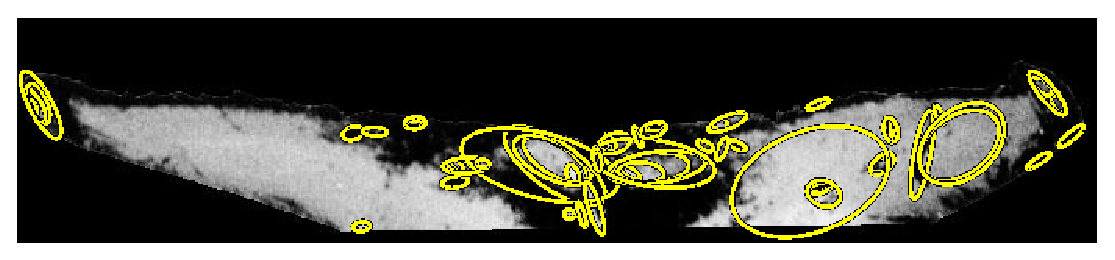
\includegraphics[width=4cm]{./Figs/mserTailA}}
\end{minipage}
\begin{minipage}[b]{0.51\linewidth}
  \centering
  \centerline{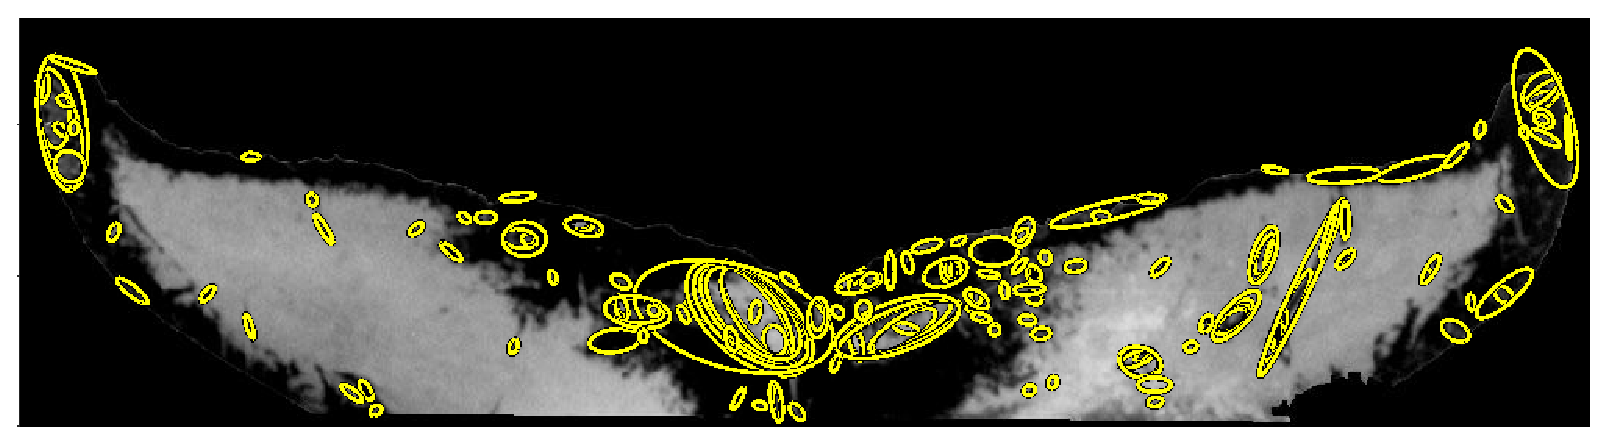
\includegraphics[width=4cm]{./Figs/mserTailB}}
\end{minipage}
\hfill
\begin{minipage}[b]{.48\linewidth}
  \centering
  \centerline{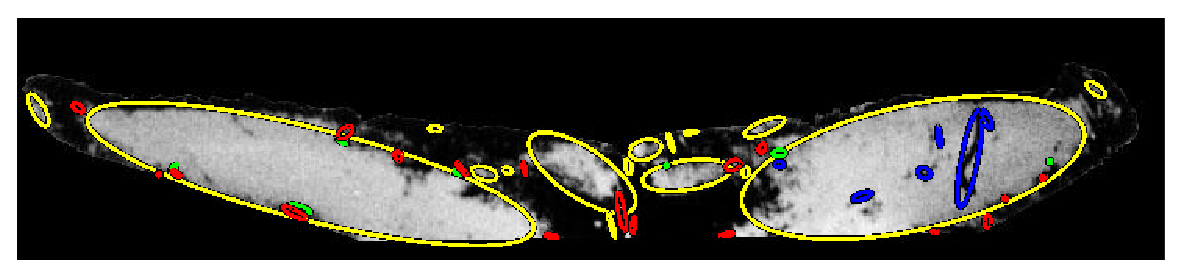
\includegraphics[width=4cm]{./Figs/dmsrTailA}}
\end{minipage}
\begin{minipage}[b]{0.51\linewidth}
  \centering
  \centerline{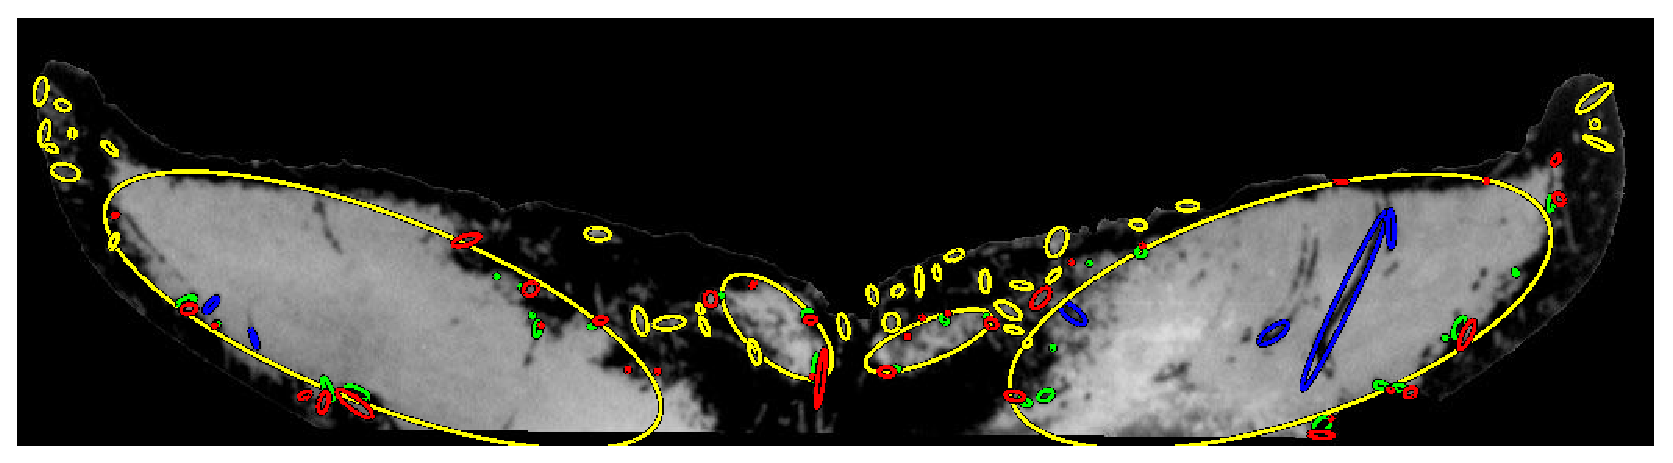
\includegraphics[width=4cm]{./Figs/dmsrTailB}}
\end{minipage}
\hfill
\vspace{-0.4cm}
\caption{Region detection on two images of the tail of the same humpback whale. 
Top row: MSER, bottom row: DMSR(All).}
\label{fig:tails}
\vspace{-0.3cm}
\end{figure}
%----------------------------------------------------------------
\begin{figure}[htb]

\begin{minipage}[b]{.24\linewidth}
  \centering
  \centerline{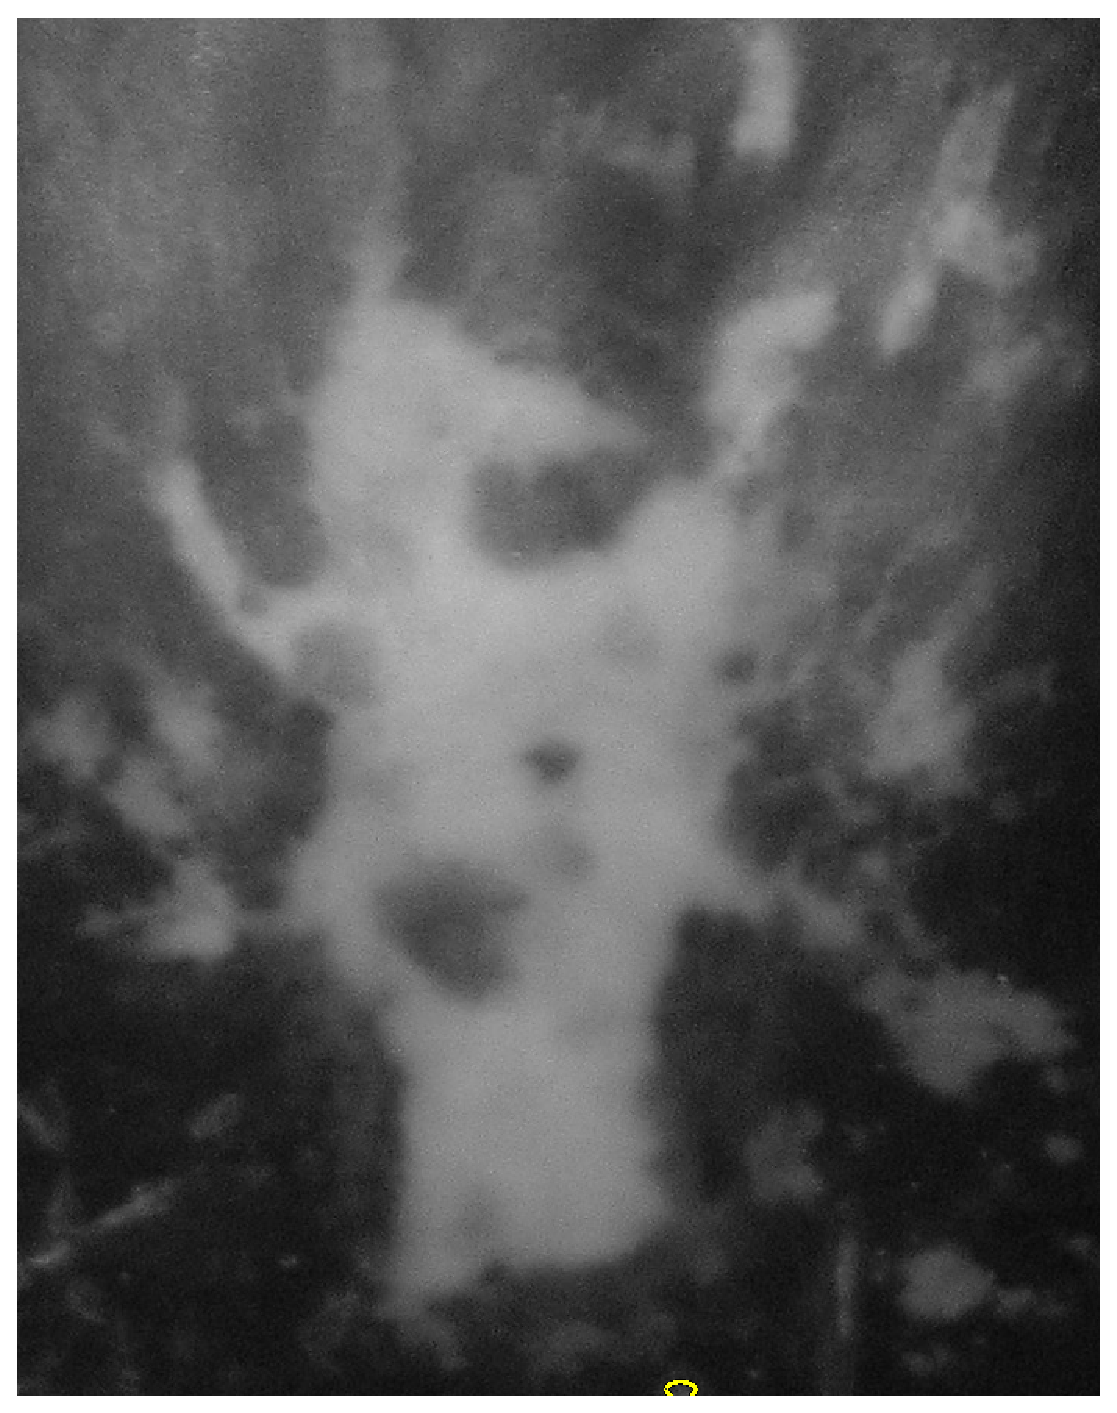
\includegraphics[width=1.8cm]{./Figs/mserLeatherbackA}}
   \centerline{(a)}\medskip
\end{minipage}
\hfill
\begin{minipage}[b]{0.24\linewidth}
  \centering
  \centerline{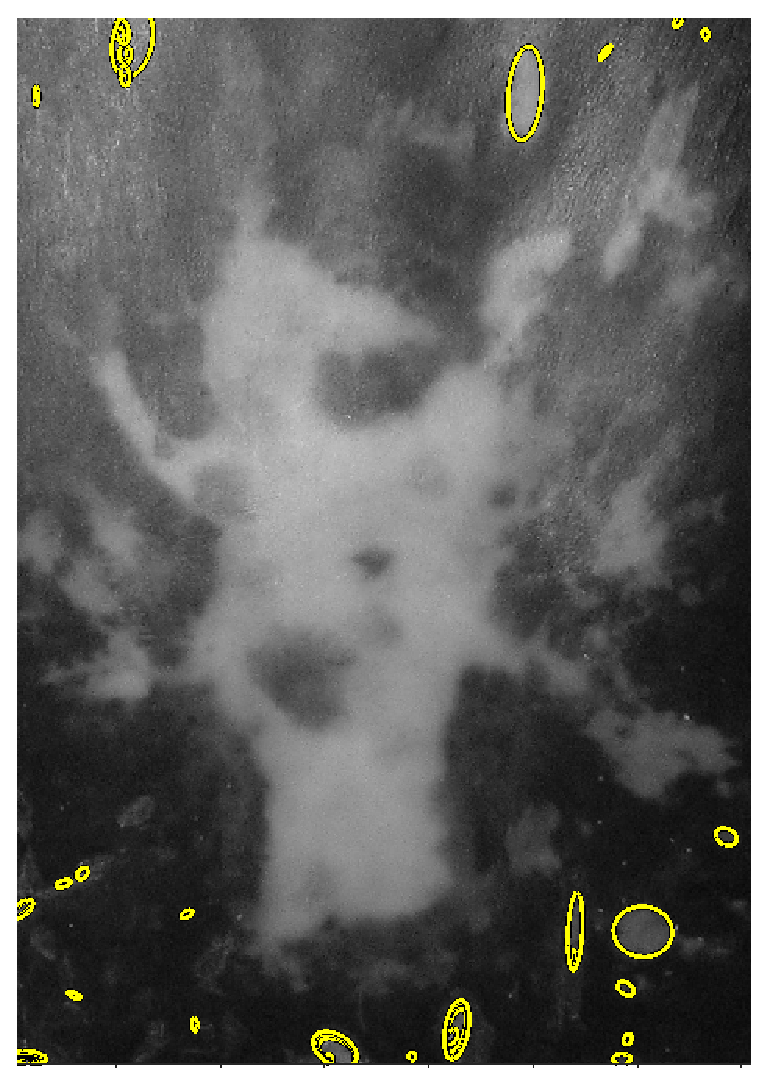
\includegraphics[width=1.8cm]{./Figs/mserLeatherbackB}}
\centerline{(b)}\medskip
\end{minipage}
\hfill
\begin{minipage}[b]{.24\linewidth}
  \centering
  \centerline{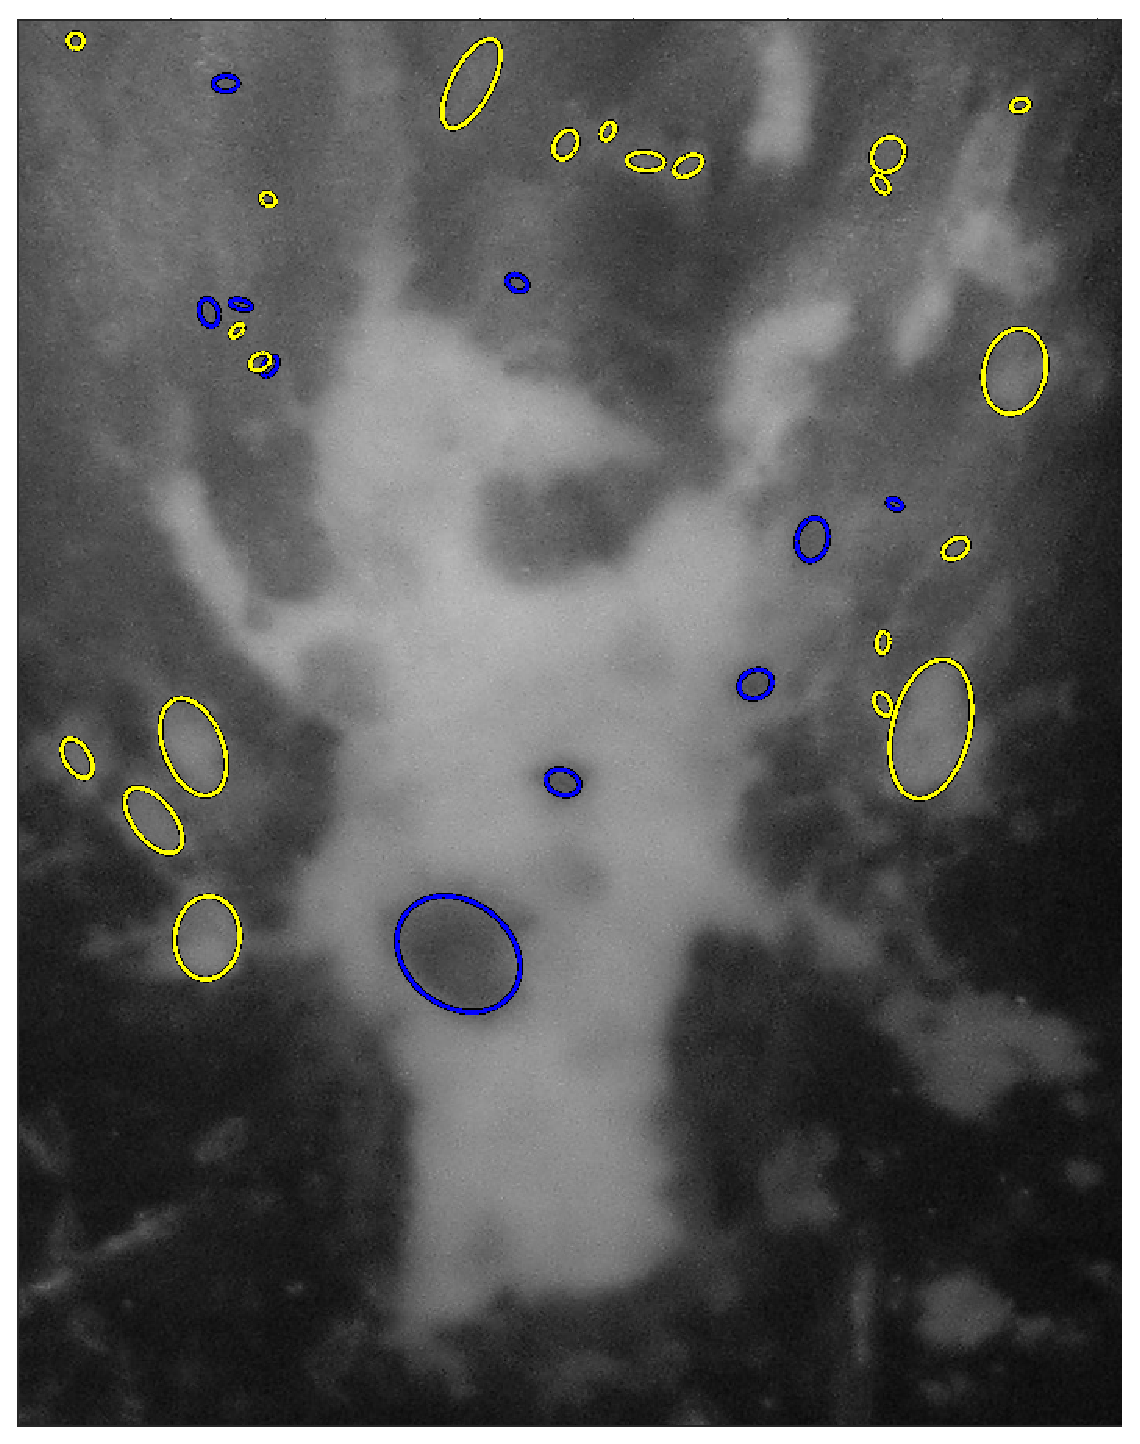
\includegraphics[width=1.8cm]{./Figs/dmsrLeatherbackA}}
\centerline{(c)}\medskip
\end{minipage}
\hfill
\begin{minipage}[b]{0.24\linewidth}
  \centering
  \centerline{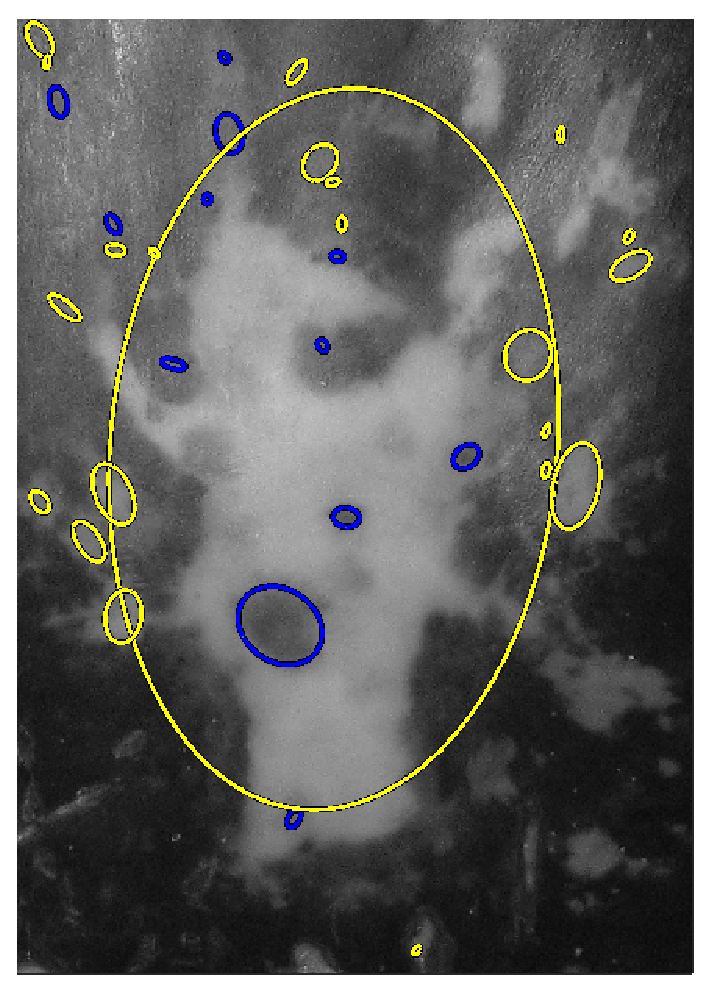
\includegraphics[width=1.8cm]{./Figs/dmsrLeatherbackB}}
 \centerline{(d)}\medskip
\end{minipage}
 \vspace{-0.2cm} 
\caption{Region detection on two images of the pineal spot of the same leatherback turtle.
(a),(b): MSER, (c),(d): DMSR.}
\label{fig:turtle}
 \vspace{-0.2cm}
\end{figure}

A decade ago, a performance evaluation paper by the Visual Geometry Group in Oxford compared existing region detectors \cite{Mikolajczyk:2005}. 
A clear conclusion of the comparison was that {\em  Maximally Stable Extremal Regions (MSER)} is the best performing detector for {\em structured} scenes \cite{Matas2002BMVC}. MSER has become the de-facto standard in the field, e.g., it is in the MATLAB CVS Toolbox and OpenCV. Despite its success, the detector has several drawbacks: sensitivity to blur, producing nested and redundant regions and degrading performance with increase of image resolution \cite{CorRos2013}. Analysis in geometric scale-space showed that the formulation of the stability criterion makes MSER prefer regular shapes \cite{Kimmel11}.

Many researchers have proposed improvements to MSER without a drastic increase of performance. An MSER color extension, {\em Maximally Stable Color Region}, outperforms both an MSER-per-color-channel combination and a color blob detector \cite{Forssen07}. Improving the MSER region distinctiveness by morphological dilation on the detected Canny edges is proposed in \cite{Wang14}. The improved detector shows better performance for bag of words classification, but evaluation of repeatability is not reported. MSER has been extended to {\em Maximally Stable Volumes} for successful segmentation of 3D medical images and paper fiber networks \cite{DonoserB06}.

%----------------------------------------------------------------------
\begin{figure}[htb]
\vspace{-0.5cm}
\begin{minipage}[b]{.49\linewidth}
  \centering
  \centerline{
\includegraphics[width=5cm]{./Figs/binary_marks}}

\end{minipage}
%\hfill
\begin{minipage}[b]{0.49\linewidth}
  \centering
  \centerline{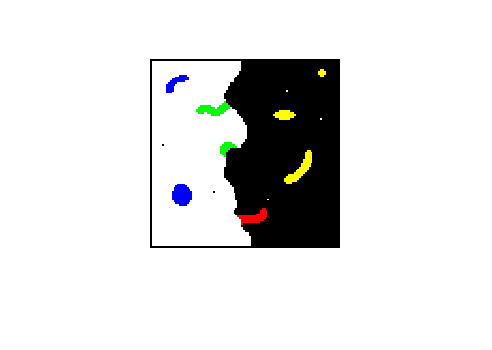
\includegraphics[width=5cm]{./Figs/binary_marks_clean_color_coded}}

\end{minipage}
\vspace{-0.5cm}
\caption{Binary salient regions detection.
Color coding: holes-blue, islands- yellow,
indentations - green, protrusions- red. }
\label{fig:binary_sal}
\end{figure}
%----------------------------------------------------------------------

Although crucial for the development of detectors, there is a shortage of evaluation benchmarks, especially for performance analysis independently of the image content. The standard {\em Oxford dataset} is very small: eight test sequences containing six (one base and five transformed) images of the same scene each. Every pair (base, transformed) is related via a given transformation matrix (homography) \cite{Mikolajczyk:2005}.  The {\em Freiburg dataset} contains $416$ higher resolution images, generated by transforming $16$ base images in order to de-tangle transformations from content \cite{FischerDB14}.  
The {\em TNT dataset} contains versions of the same viewpoint sequences with increasing resolution from $1.5$ to $8$~MPixel per image. Highly accurate image pair homographies are given. It is suitable for evaluating robustness to resolution rather than to transformations \cite{CorRos2013}. 

This paper contributes to solving the identified problems. A new regions detector, {\em Data-driven Morphology Salient Regions (DMRS)} is proposed and made available as open source \cite{elena_ranguelova_2016_45156}. It is related to the {\em Morphology-based Stable Salient Regions (MSSR)} detector that we developed in the context of humpback whale identification \cite{RangMSSR06, RangHumpb06}. DMRS includes a binarization, %robust-to-lighting-and-blur
that yields a much smaller number of regions and is more stable across transformations. It has similar or higher (lighting, blur and increased resolution) repeatability compared to MSER, while detecting % non-redundant 
perceptually salient regions (Fig.~\ref{fig:tails}). Figure\,\ref{fig:turtle} (c), (d) illustrates that DMSR finds salient regions repeatedly on the leatherback turtle images, unlike MSER. Also, we made an openly available dataset, OxFrei, combining the natural homographies of the Oxford and the higher resolution images of the Freiburg datasets \cite{elena_ranguelova_2016_45156}.

\section{Data-driven Morphology Salient Regions Detection}
\label{sec:DMSR}

MSER and MSSR decompose a gray-scale image into binary cross-sections and evaluate the stability of the connected components (CCs) or accumulate saliency masks. DMSR starts with a data-driven binarization, producing one binary image, thus transforming the problem into binary saliency.

%----------------------------------------------------------------------
\begin{table}[hbt]
\begin{minipage}[b]{0.99\linewidth}\begin{tabular}{|l l|}
\hline
{\bf ISS} & A CC $S^i_{fb} = \{\p \in \mcD, \forall \p=foreground,$\\&$\forall \q \in \partial S^i_{fb}, \q=background, \q \notin \partial \B $ \},\\
$2$ types & $S^i_{10}$ (islands), $S^i_{01}$  (holes); $\S^i = S_{01}^i \cup S_{10}^i$\\
{\bf BSS} &  $S_{fb}^b: \{\p \in S_{fb}^b \subset{\cal B}^f, \forall \p = foreground,$\\&$ \q \in \partial S_{fb}^b \subset {\partial \cal B}^f,\forall \q = background \}$, \\
& $|\partial {\cal B}^f| - |\partial ({\cal B}^f \backslash S_{fb}^b)| < 2 \pi r$\\
$2$ types & $S^b_{10}$ (protr.), $S^b_{01}$ (indent.); $\S^b = S_{01}^b \cup S_{10}^b$\\
{\bf Regions} &  $\S = \S^i$ (DMSR); $\S = \S^i \cup \S^b$ (DMSRA)  \\
\hline
\end{tabular}
\hfill
\centering
\caption{Binary saliency definitions used in Section \ref{ssec:binary}.}\label{table:binary_sal}
\end{minipage}
\vspace*{-0.4cm}
\end{table}


\subsection{Binary Salient Regions Detection}
\label{ssec:binary}
We claim that the perceptual saliency in a binary image of a structured scene 
 $\B: \mcD \subset \mathcal{Z}^2 \rightarrow \{0,1\}$ (1-white, 0-black)
is only due to the spatial layout of the image regions \cite{RangHumpb06}. 
There are  $4$ types of salient regions. The $2$ types of {\em inner salient structures (ISS)} are (1) {\em holes} -- set of connected black pixels entirely surrounded by white pixels, and (2) {\em islands} -- set of connected white pixels surrounded by black ones, i.e.~inverse of holes. A significant connected component ${\cal B}^1$ is defined as a CC with area proportional to the image area by $\Lambda$. The radius of the morphological structuring element is $r$ and  the area opening parameter for  noise filtering is $\lambda$. The $2$ {\em boundary salient structures (BSS)} are (3) {\em protrusions}- set of white pixels on the border of a significant CC, which if pinched off from the CC, will increase its boundary with no more than $2\pi r$, and (4) the {\em indentations}- protrusions inverse. 


The types are also valid for the MSSR detector. The regions are obtained from $\B$ by morphological operations: hole filling, top hat and area opening, for details see \cite{RangMSSR06, RangHumpb06}. The ISS are similar to the definition of the MSER+ and MSER- regions \cite{Matas2002BMVC}. In this paper, detectors using only ISS, i.e., directly comparable to MSER, are denoted by DMSR/MSSR, while DMSRA/MSSRA are detectors using all region types. These definitions are summarized in Table~\ref{table:binary_sal} and the exact shaped regions from a synthetic $100 \times 100$ binary image with parameters $\Lambda=100$, $r=5$ and $\lambda = 10$ are shown on Fig.~\ref{fig:binary_sal}.

\subsection{Data-driven binarization}
\label{ssec:binarize}
Any gray-scale image  $\I:~\mcD~\subset~\mathcal{Z}^2~\rightarrow ~\mcT $, where $\mcT=\{0,1,\ldots, t_{max}\}$ and $t_{max}~=~2^n-1~=~255$ is the maximum gray value encoded by $n~=~8$ bits, can be decomposed into cross-sections at
every possible level $t$:  $\I = \sum_{t \in \mcT}CS_t(\I)$. Obtaining a section at level $t$ is equivalent to thresholding the image at threshold $t$: $CS_t(\I)= 1.(\I>t) + 0.(\I<t)$ is a binary image. 
Three sets of connected components in $CS_t(\I)$ are defined: $\mcA_t$- {\em all}, $\mcL_t$- the {\em large} and $\mcV_t$- the {\em very large} CCs.  The size of each CC category is defined by$\Lambda_{\mcL}$ and $\Lambda_{\mcV}$ fraction of the image area $A_{\I}$. Let us denote the normalized number of elements in a set ($|\cdot|$) by $\Vert \cdot \Vert = |\cdot| / \max_{t \in \mcT}|\cdot|$.
Finding the optimal threshold $t_{opt}$ is then defined as:
\begin{equation*}
\vspace{-0.05cm}
t_{opt} = \argmax_{t \in \mcT}( w^{\mcA} \Vert \mcA_t \Vert + w^{\mcL} \Vert \mcL_t \Vert + w^{\mcV} \Vert \mcV_t \Vert ),
\vspace{-0.05cm}
\end{equation*}
where $w^{\cdot}$ are the weights per set of CCs.  

The standard Otsu thresholding does not select a single stable $CS$, while choosing $t_{opt}$ ensures stable number of regions across transformations (see Figs.~\ref{fig:binary_hist} and \ref{fig:leuven_bin} for lighting).
%------------------------------------------------------------------------
\vspace{-0.8cm}
\begin{figure}[htb]

\begin{minipage}[b]{0.49\linewidth}
  \centering
  \centerline{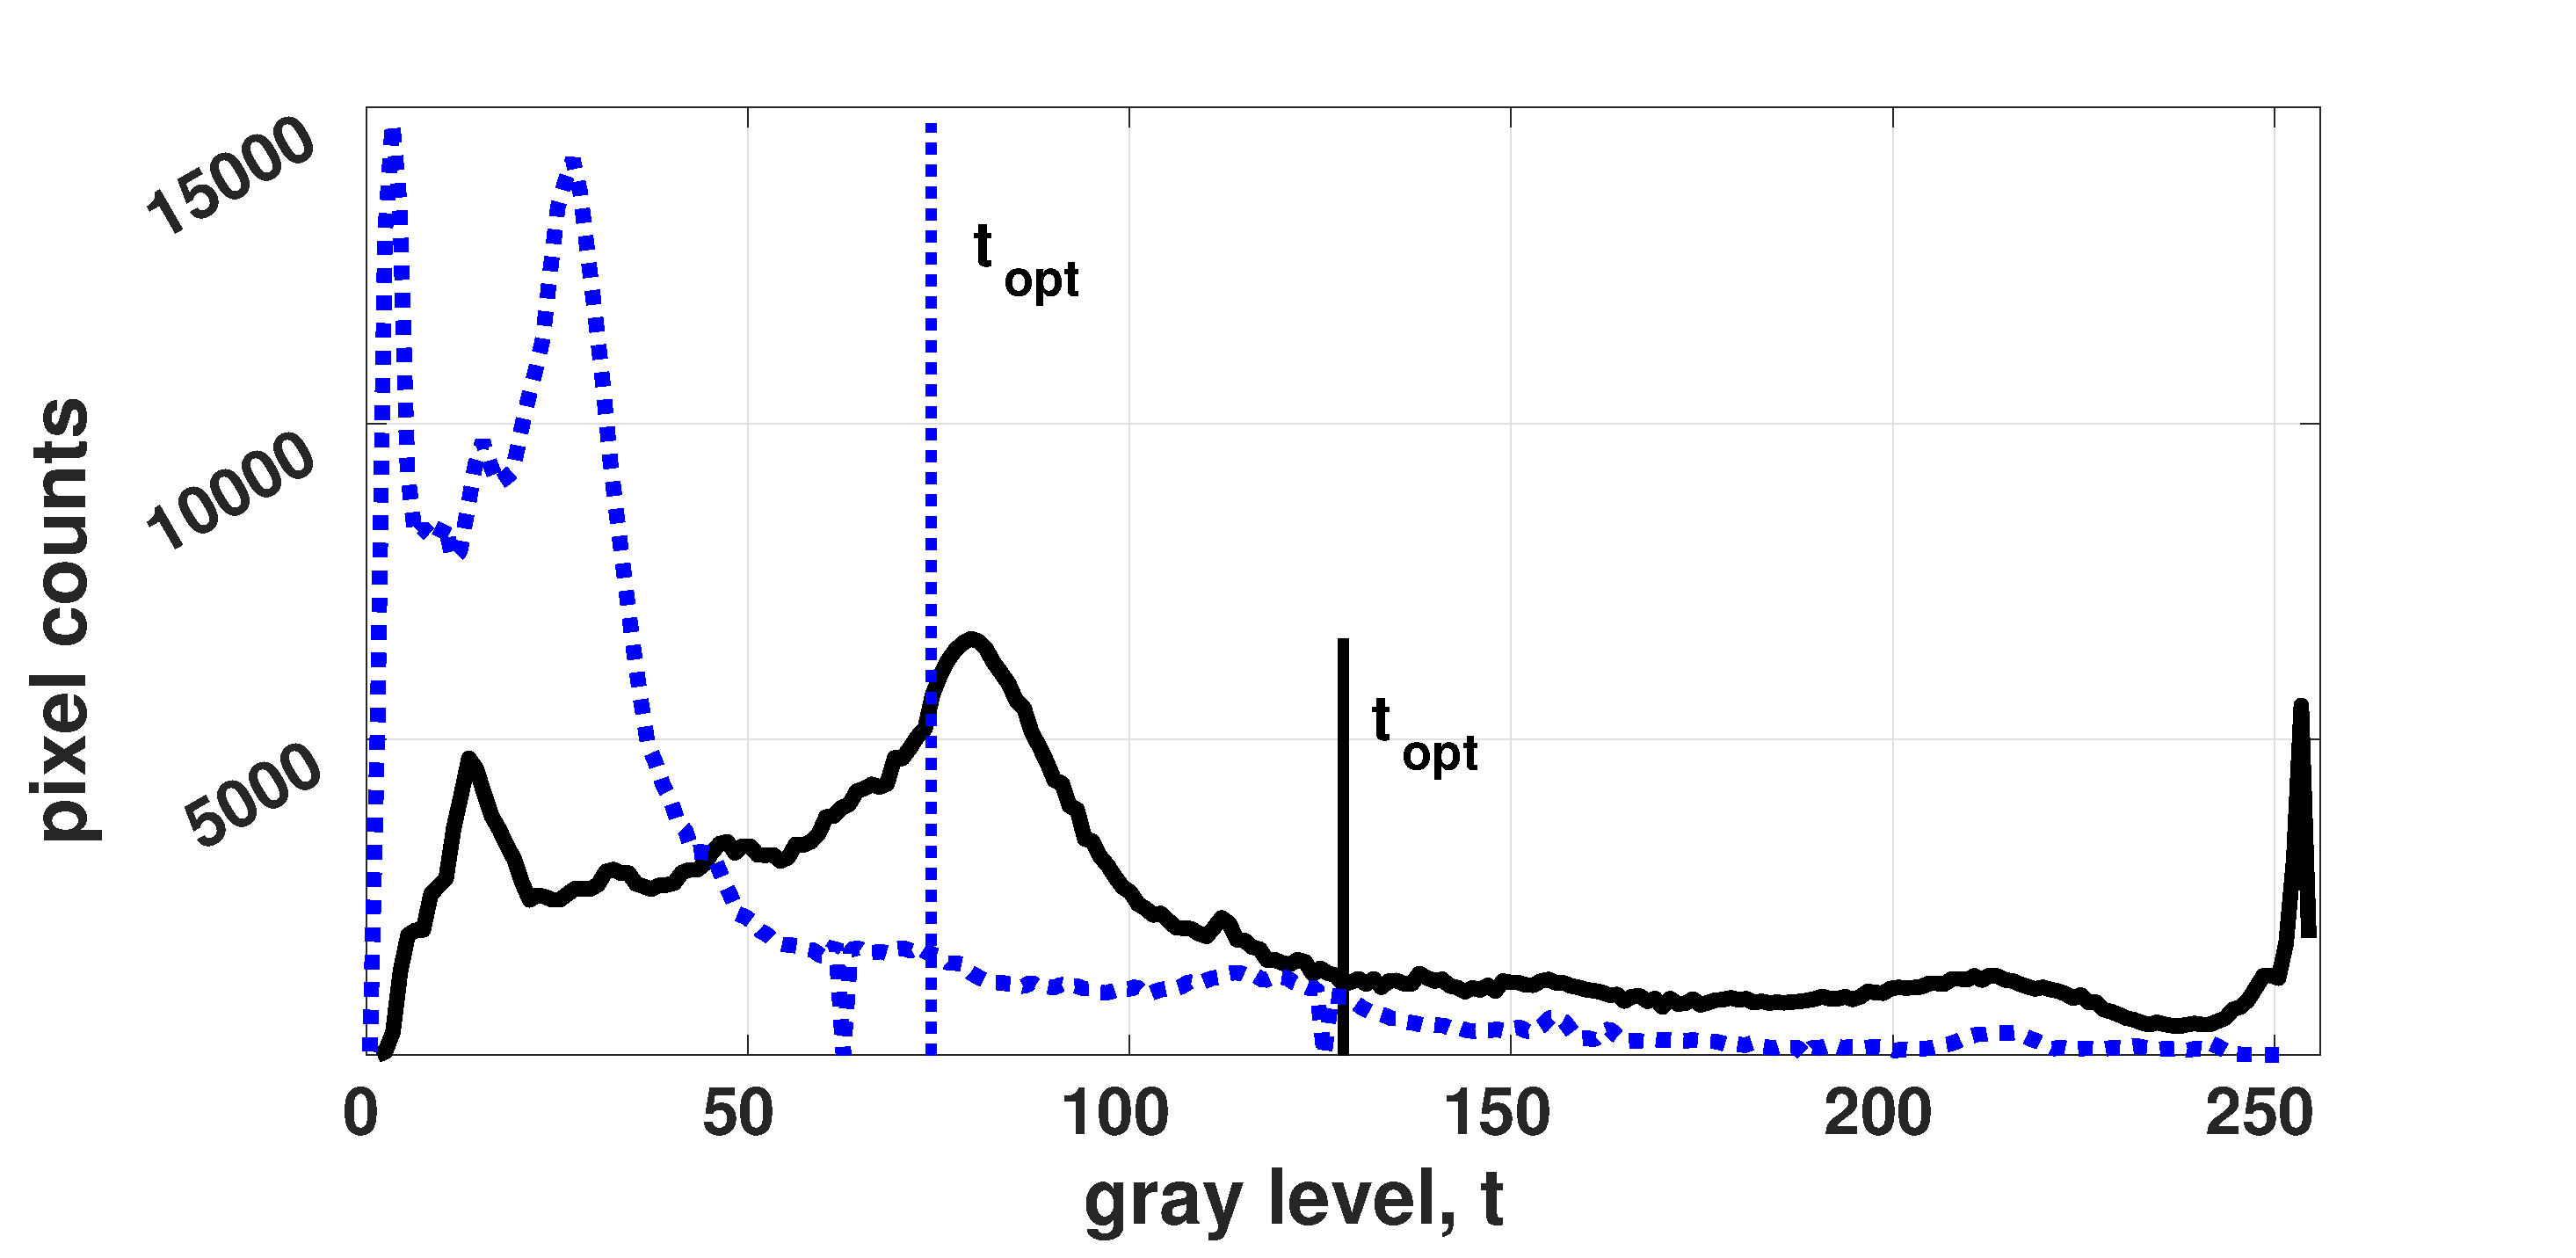
\includegraphics[width=4.65cm]{./Figs/hist_otsu_leuven_1_4}}
  \centerline{(a) Otsu}\medskip
\end{minipage}
\hfill
%\vspace{-0.5cm}
\begin{minipage}[b]{0.49\linewidth}
  \centering
  \centerline{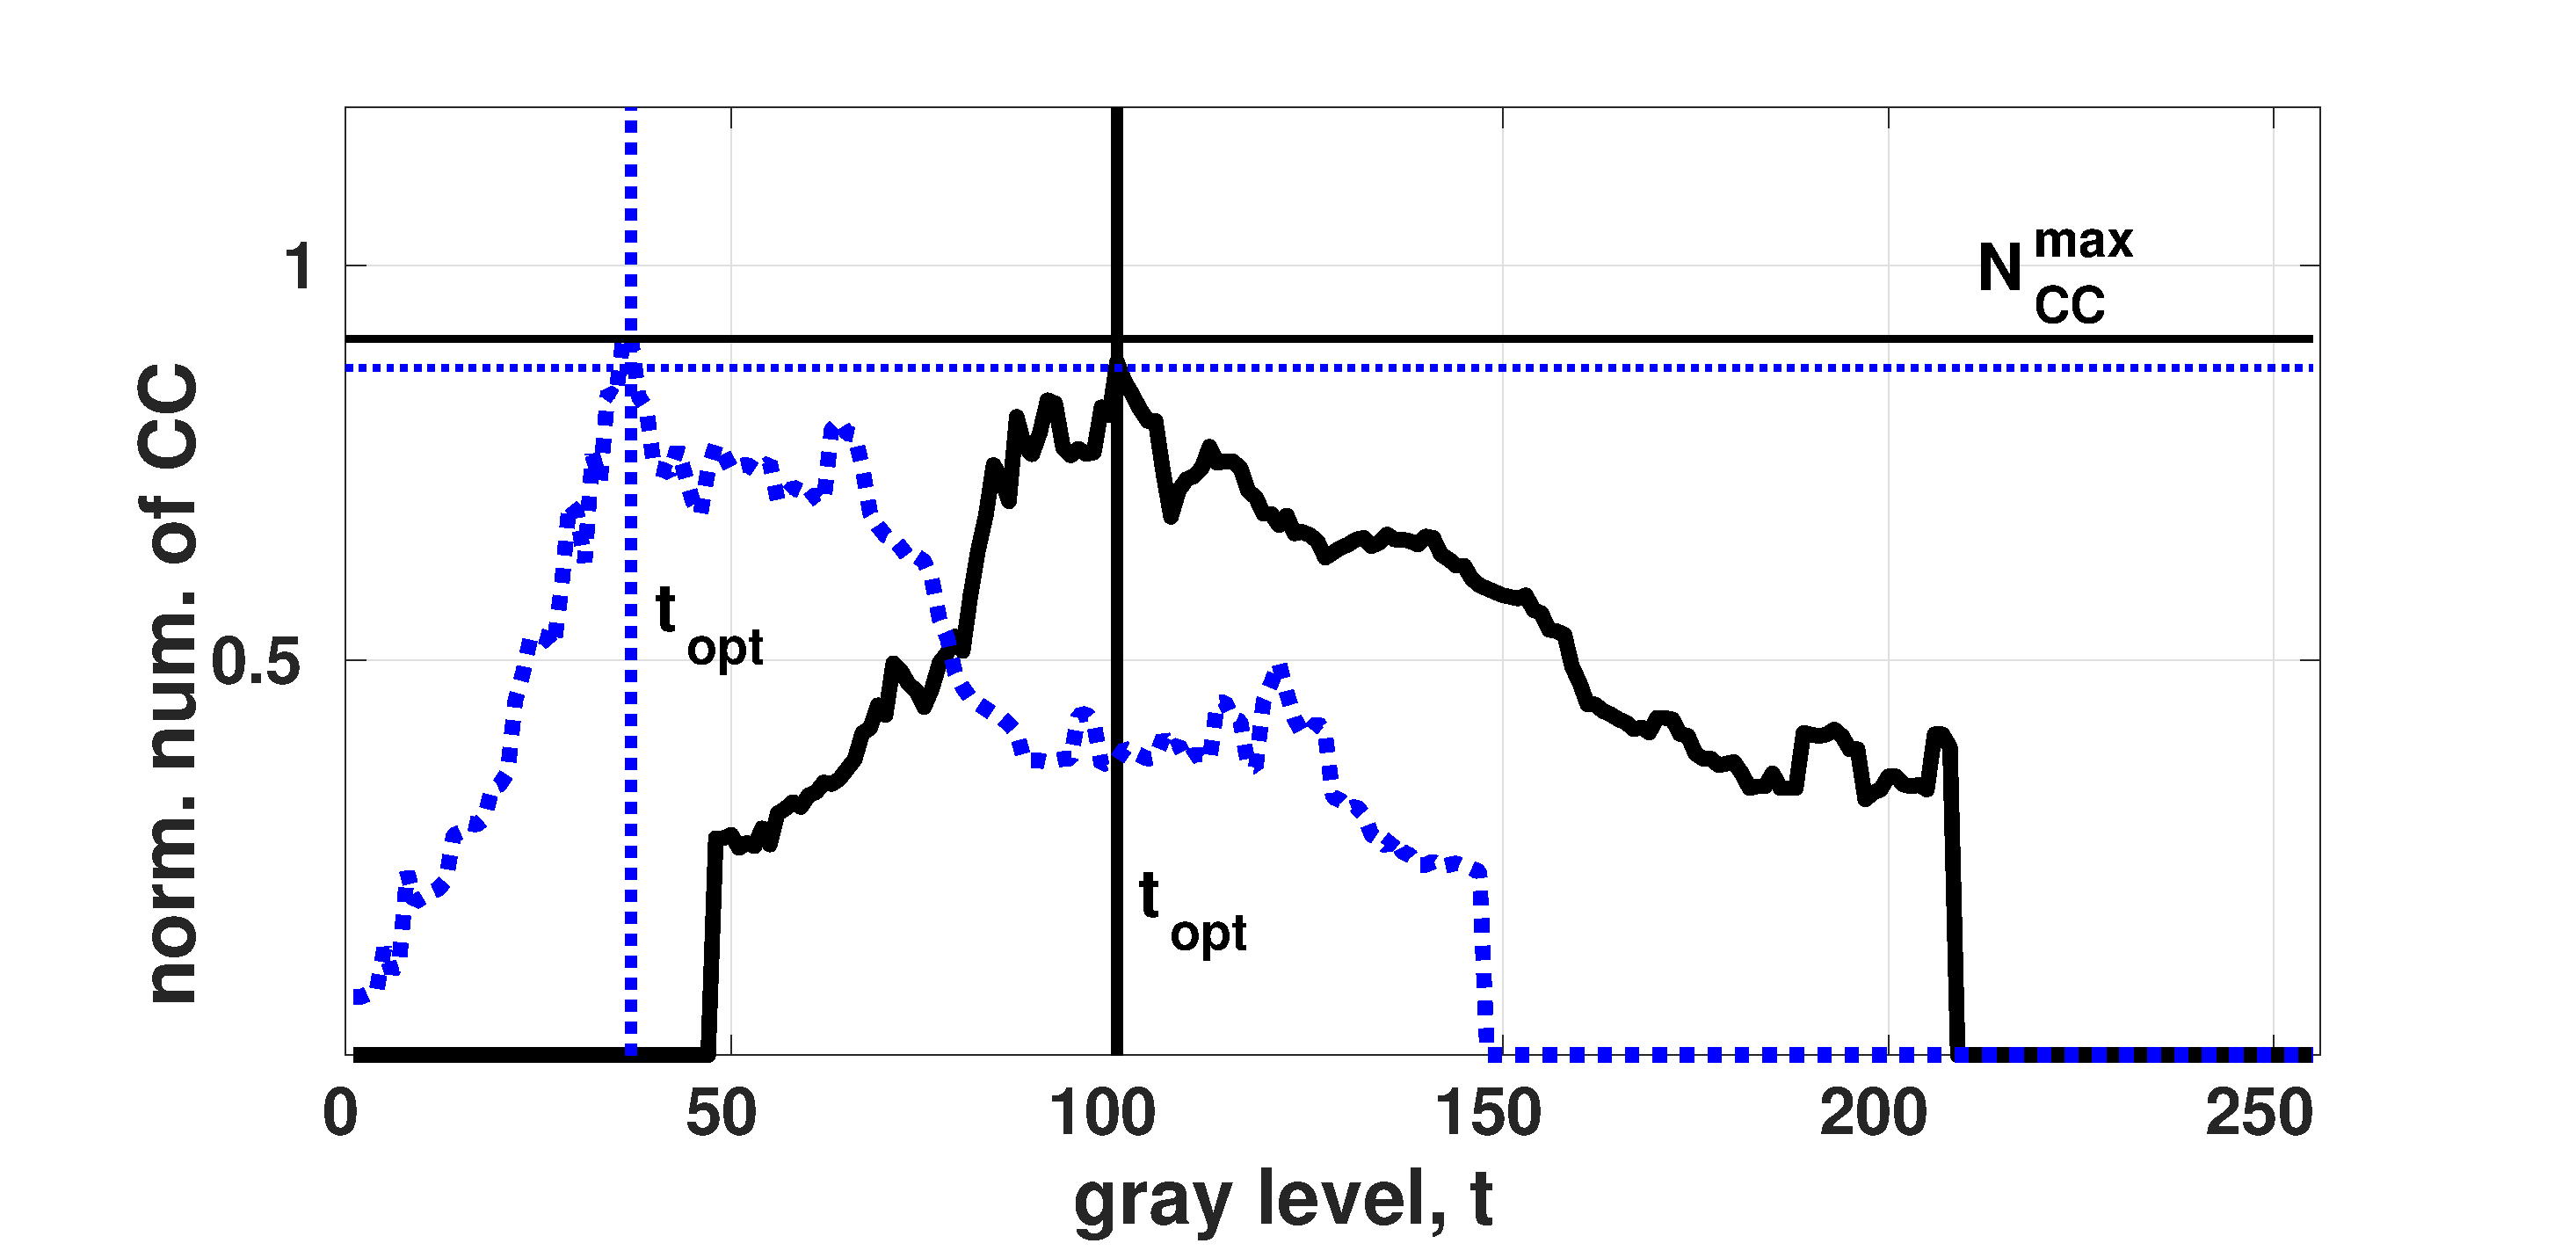
\includegraphics[width=4.8cm]{./Figs/hist_numcc_leuven_1_4}}
\centerline{(b) Max number CC}\medskip
\end{minipage}
\hfill
\vspace{-0.5cm}
\caption{Finding the optimal threshold for two images from the 'Leuven' sequence 
(Oxford dataset, lighting): the base image- solid black line, the forth image - dotted blue line.}
\label{fig:binary_hist}
%
\end{figure}
%------------------------------------------------------------------------
%\vspace{-0.5cm}

\begin{figure}[htb]

\begin{minipage}[b]{.3\linewidth}
  \centering
  \centerline{\includegraphics[width=2.8cm]{./Figs/leuven1}}
%  \vspace{1.5cm}
%   \centerline{(a)}\medskip
\end{minipage}
\hfill
\begin{minipage}[b]{0.3\linewidth}
  \centering
  \centerline{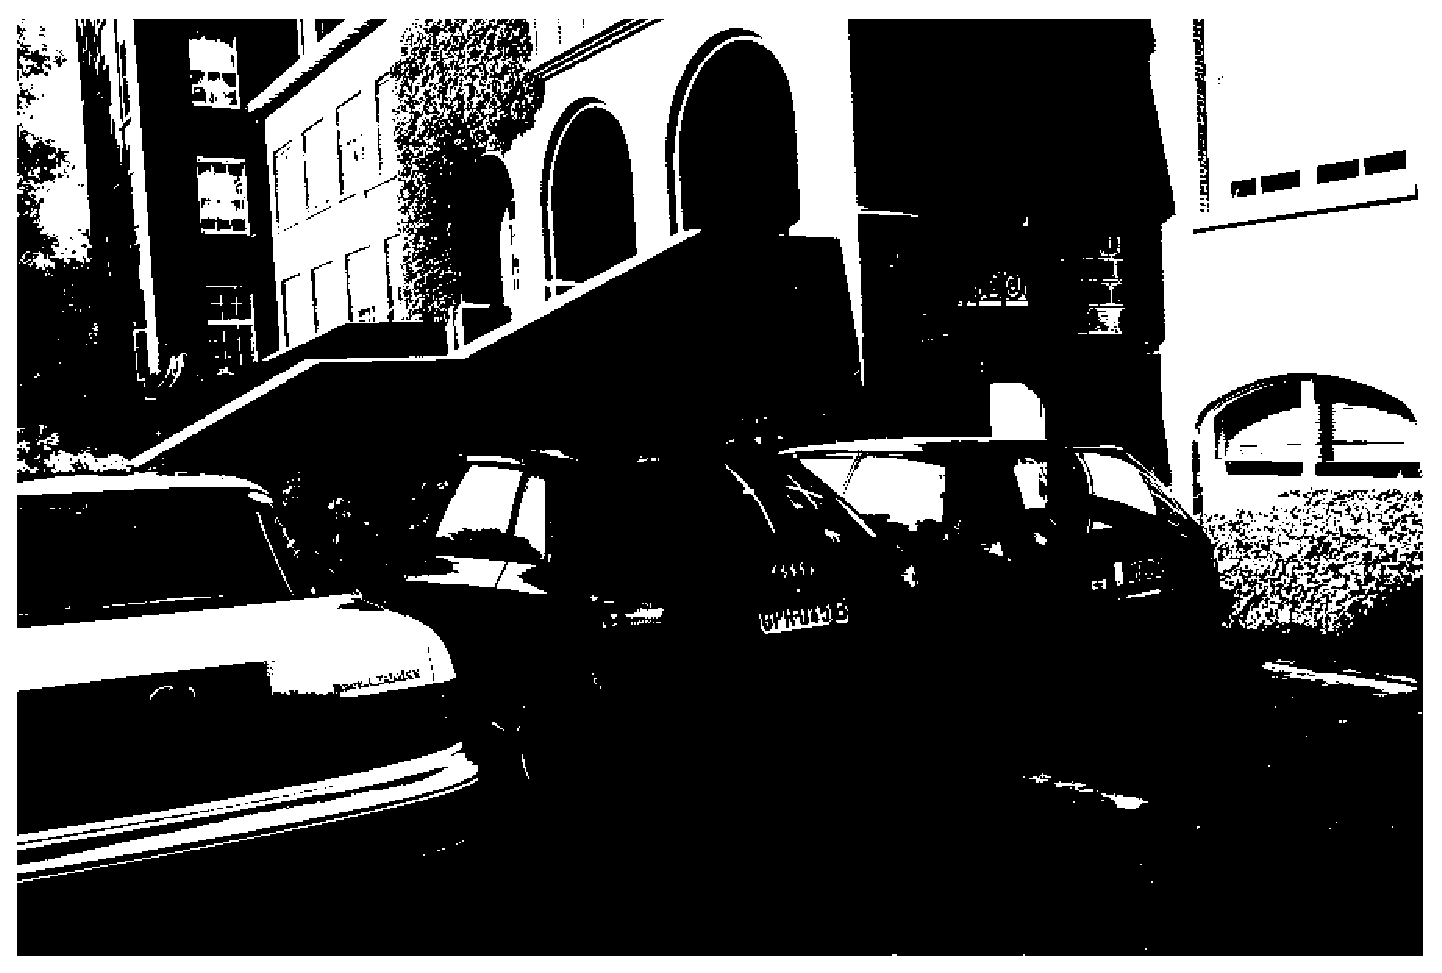
\includegraphics[width=2.7cm]{./Figs/leuven1_otsu}}
%  \vspace{1.5cm}
  % \centerline{(b)}\medskip
\end{minipage}
\hfill
\begin{minipage}[b]{0.3\linewidth}
  \centering
  \centerline{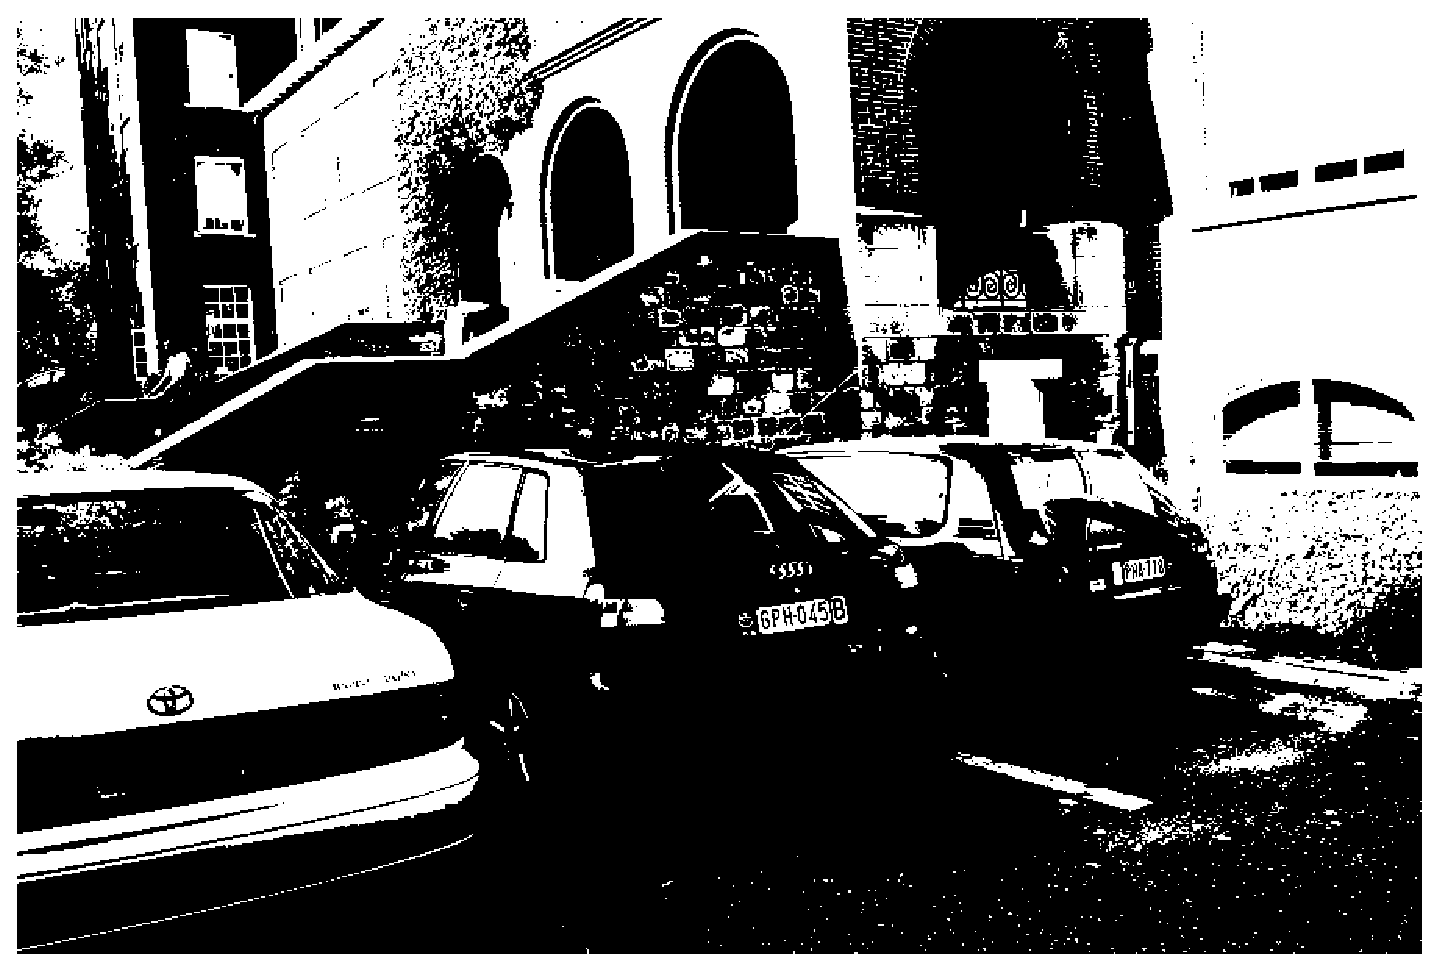
\includegraphics[width=2.7cm]{./Figs/leuven1_numcc}}
%  \vspace{1.5cm}
  % \centerline{(c)}\medskip
\end{minipage}

\begin{minipage}[b]{.3\linewidth}
  \centering
  \centerline{\includegraphics[width=2.7cm]{./Figs/leuven4}}
%  \vspace{1.5cm}
   \centerline{(a)}\medskip
\end{minipage}
\hfill
\begin{minipage}[b]{0.3\linewidth}
  \centering
  \centerline{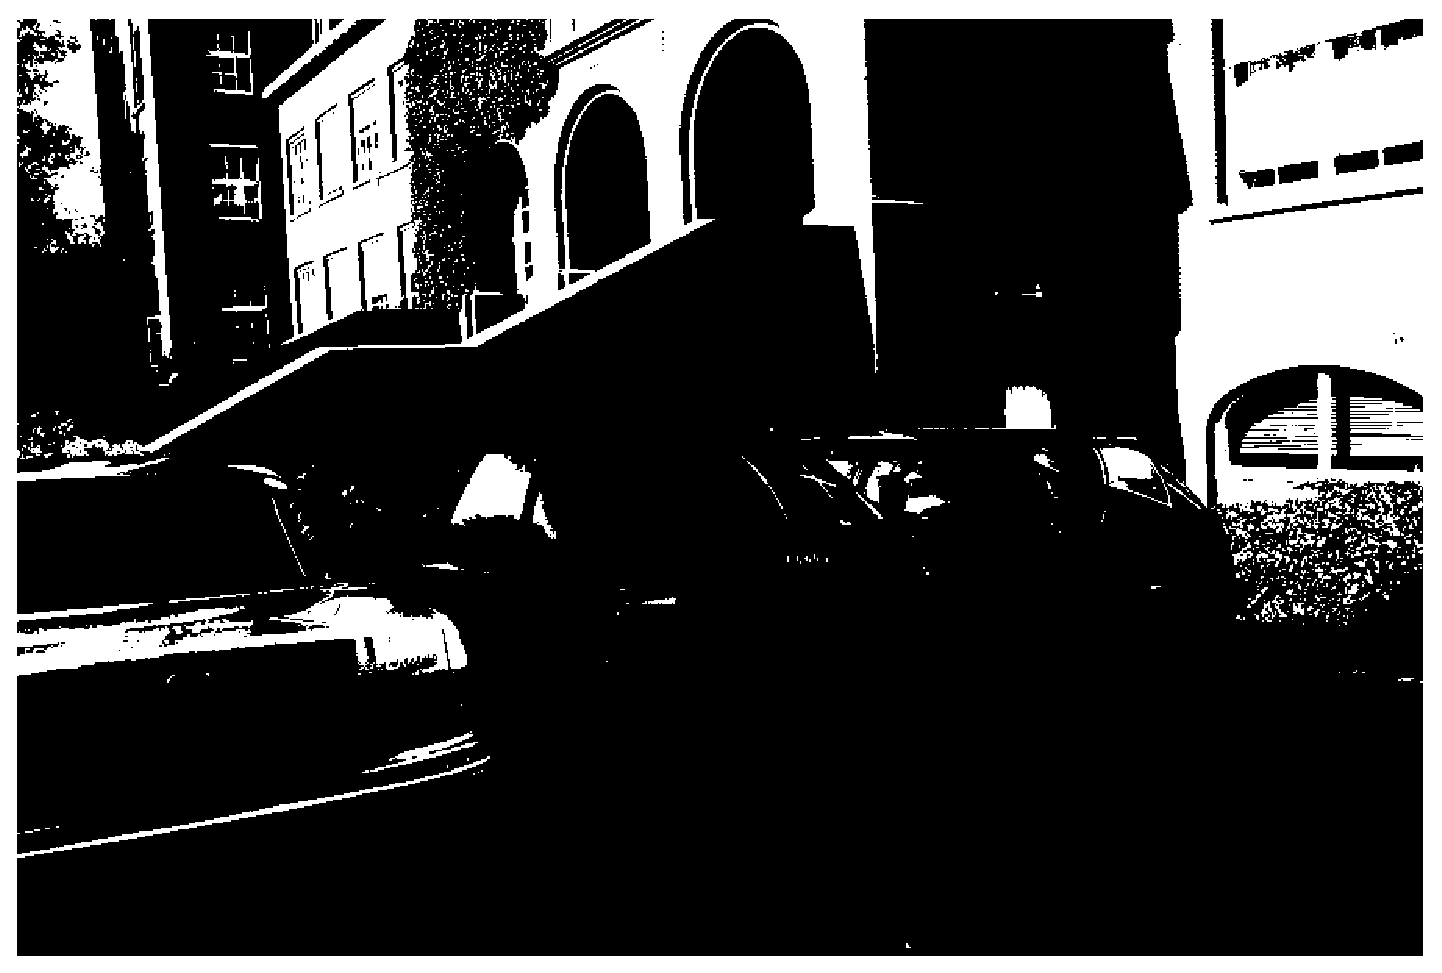
\includegraphics[width=2.7cm]{./Figs/leuven4_otsu}}
%  \vspace{1.5cm}
   \centerline{(b)}\medskip
\end{minipage}
\hfill
\begin{minipage}[b]{0.3\linewidth}
  \centering
  \centerline{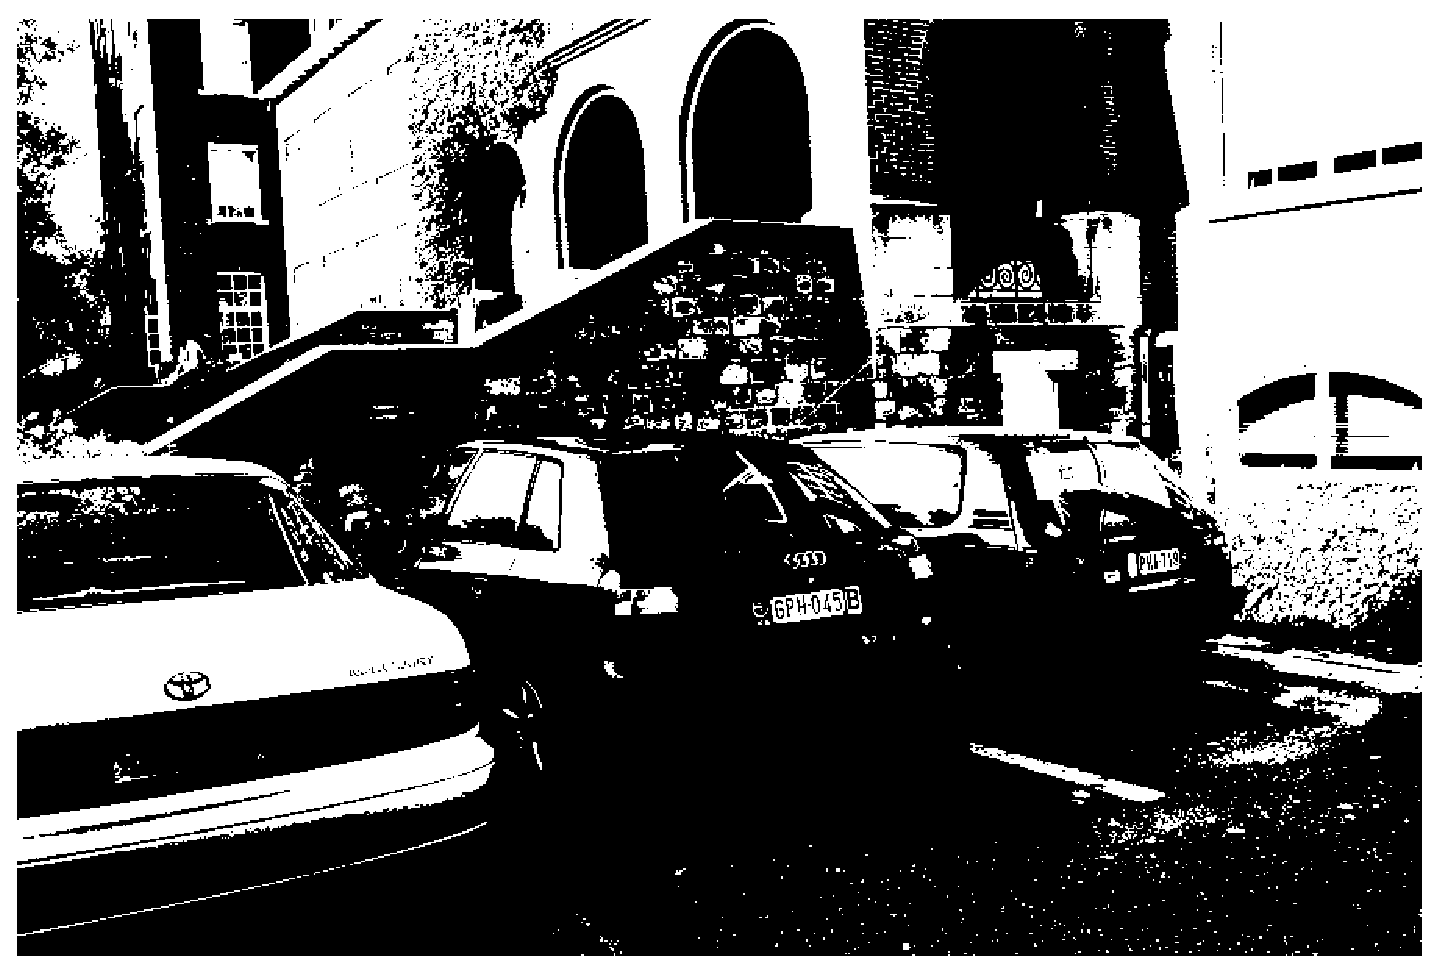
\includegraphics[width=2.7cm]{./Figs/leuven4_numcc}}
%  \vspace{1.5cm}
   \centerline{(c)}\medskip
\end{minipage}

 \vspace{-0.5cm}
\caption{Binarization of two images of the 'Leuven' sequence (lighting). Top row- base image, bottom row- forth image;   (a) gray scale; (b) Otsu binarization, (c) proposed binarization.}
\label{fig:leuven_bin}
%
\end{figure}
%------------------------------------------------------------------------

After the data-driven binarization, the DMSR detector finds the set of affine-covariant regions $\S$ from the single binary image $CS_{t_{opt}}$ as described in Section \ref{ssec:binary} and \cite{RangMSSR06, RangHumpb06}. DMSR produces fewer non-overlapping and perceptually salient regions (visualized by their equivalent ellipses, not exact shapes) compared to MSER (see Figures~\ref{fig:det_graffiti} and \ref{fig:wood}).

\section{Performance  Evaluation}
\label{sec:perf}
The {\em repeatability score} ($R$) and the {\em number of correspondences} ($N_C$) are the main performance evaluation measures \cite{Mikolajczyk:2005}. The maximum overlap error between matching regions is $40\%$. The $R$ score between a pair of base and transformed image, $(\I_B,\I_T)$, is the ratio between $N_C$ in the common image part and the smaller number of regions in the pair. The structured scenes from each dataset are considered and five detectors are evaluated: MSER, MSSR(A) and DMSR(A). The MSER software is used with its default settings and the (D)MSSR(A) parameters are: $r = 0.02*\sqrt{A_{\I} / \pi}$, $\lambda=3r$, $\Lambda_{\mcL}=0.001$, $\Lambda_{\mcV}=0.01$ and  $w^{\cdot}=0.33$.  
All performance plots and detected regions on all data are available online \cite{elena_ranguelova_2016_45156}.

%------------------------------------------------------------------------
\begin{figure}[htb]

\begin{minipage}[b]{.49\linewidth}
  \centering
  \centerline{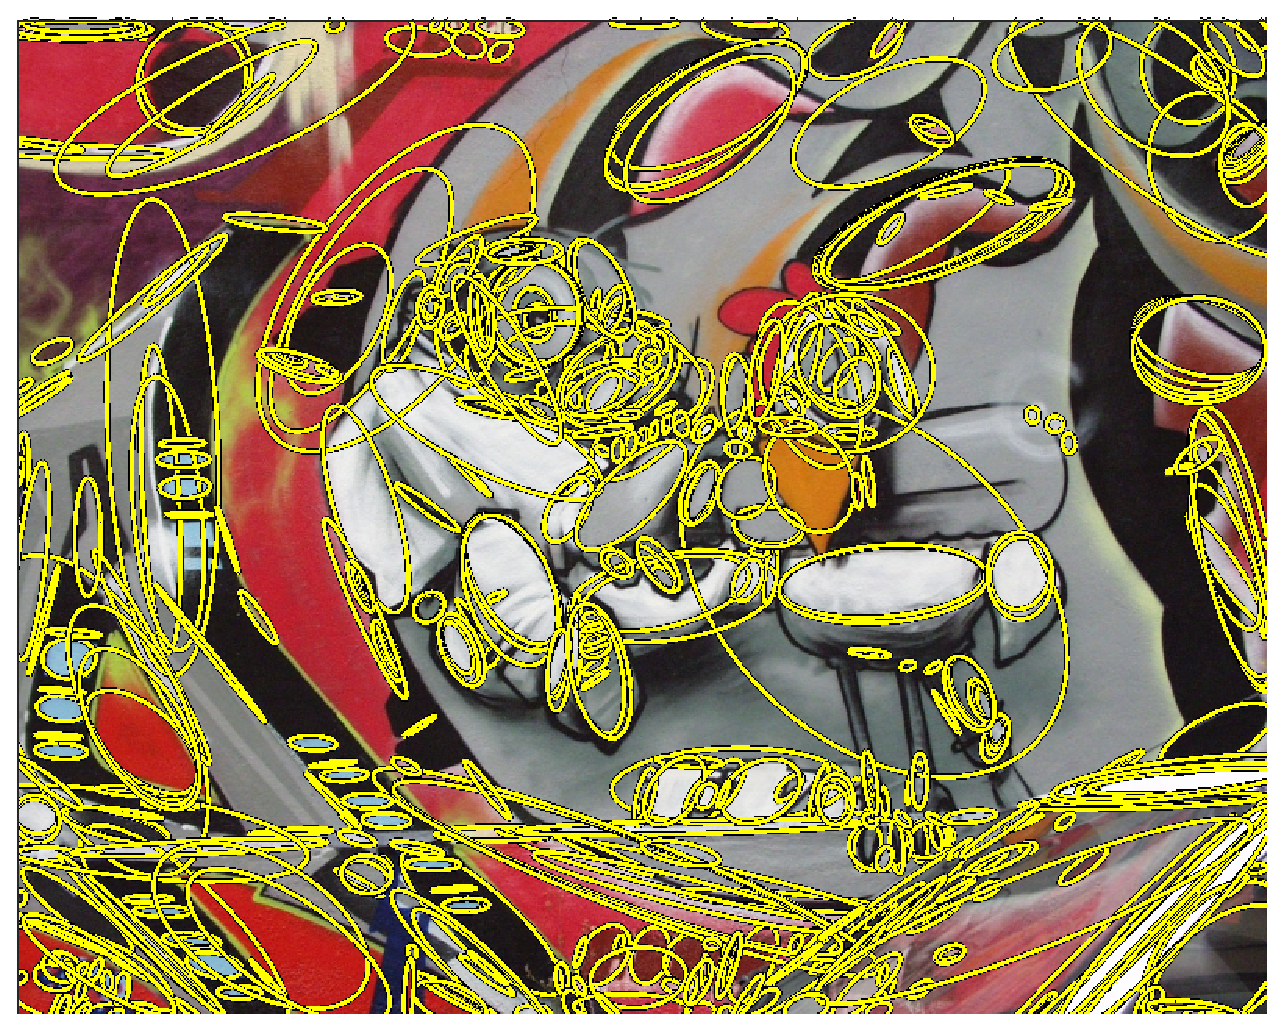
\includegraphics[width=4.0cm]{./Figs/mserGraffiti1}}
 % \vspace{0.2cm}
 % \centerline{(a) MSER}\medskip
\end{minipage}
\hfill
\begin{minipage}[b]{0.49\linewidth}
  \centering
  \centerline{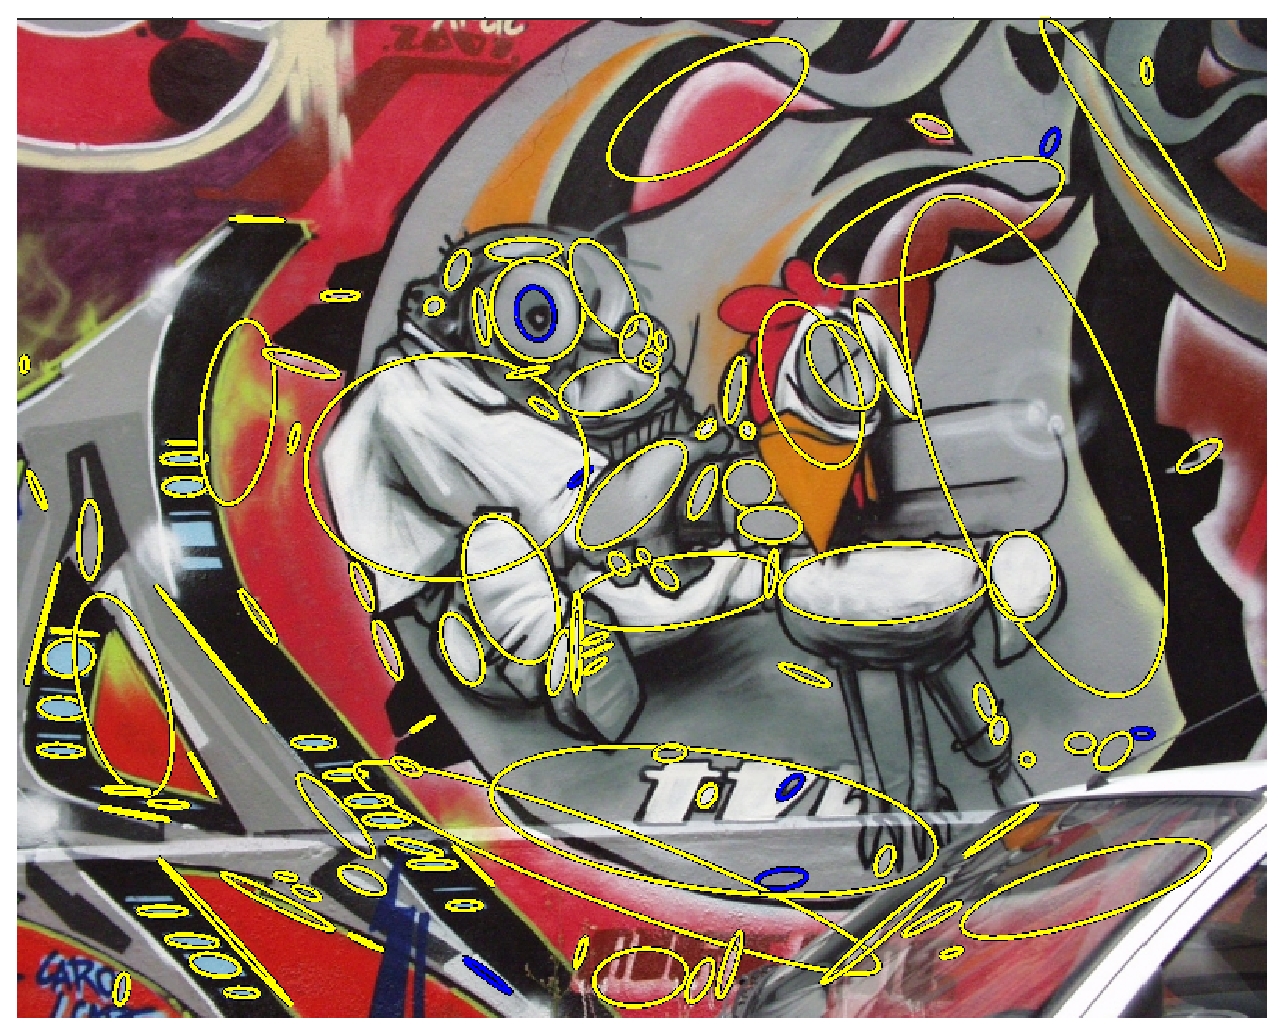
\includegraphics[width=4.0cm]{./Figs/dmsrGraffiti1}}
 % \vspace{0.2cm}
 % \centerline{(b) DMSR}\medskip
\end{minipage}
\vspace{-0.25cm}
\caption{Region detectors on the base image of the 'Graffiti' sequence, Oxford dataset. Left: MSER, right: DMSR}
\label{fig:det_graffiti}
%
\end{figure}
%------------------------------------------------------------------------
\begin{figure}[htb]

\begin{minipage}[b]{.49\linewidth}
  \centering
  \centerline{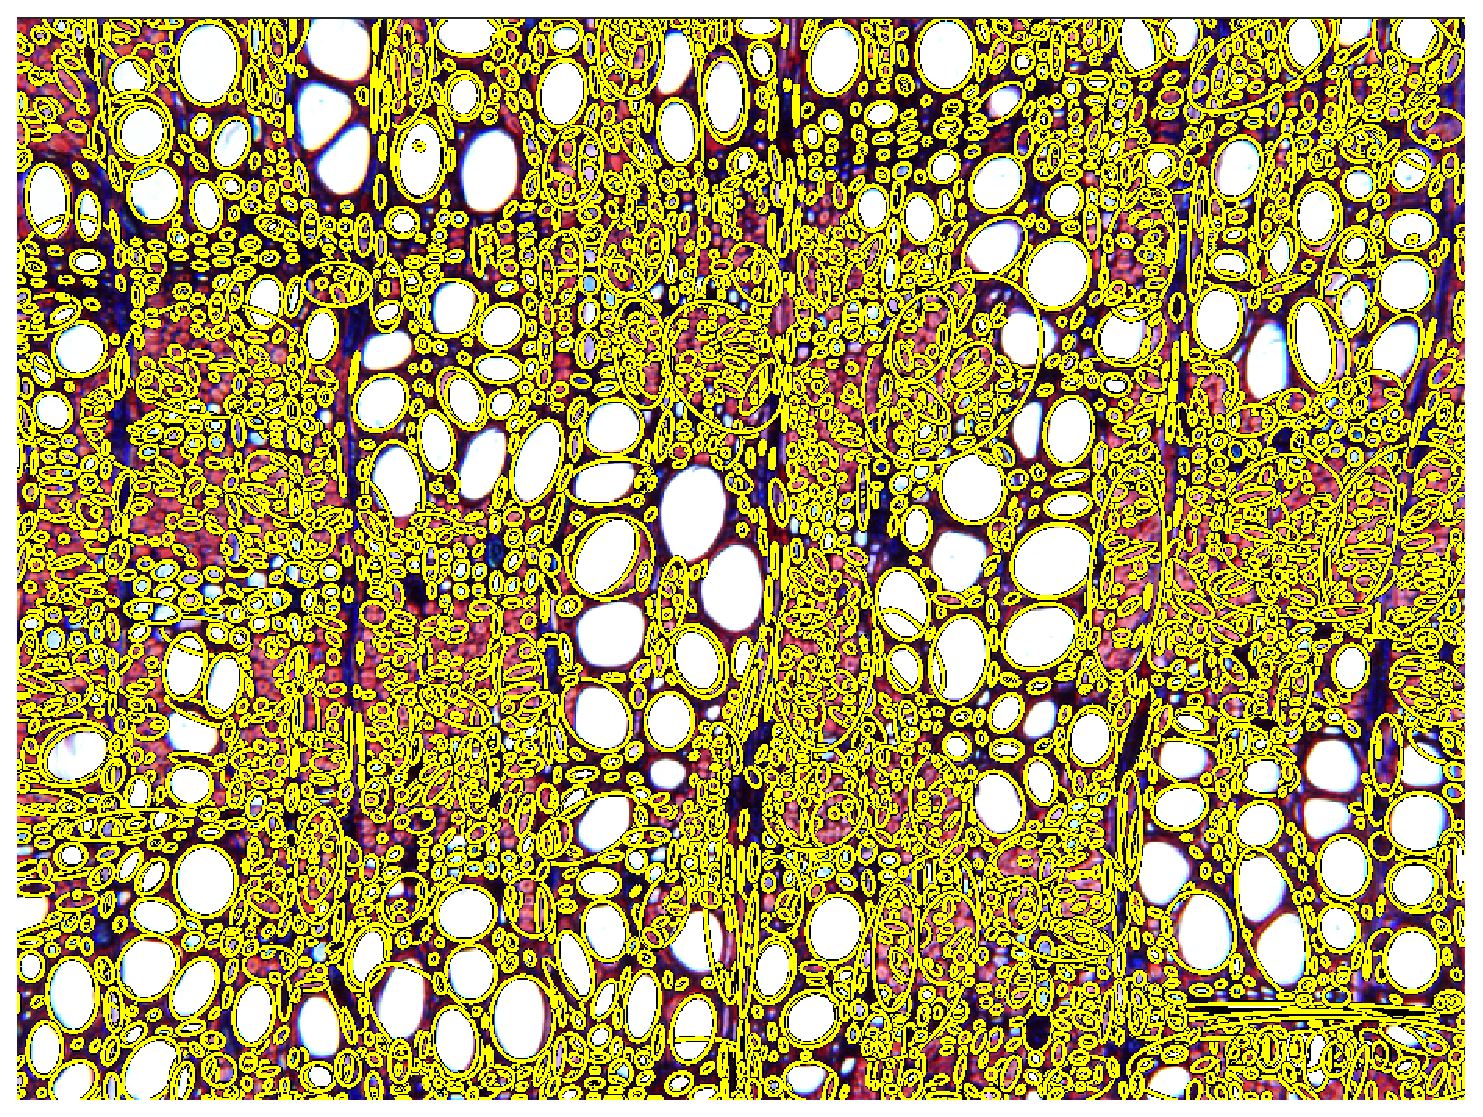
\includegraphics[width=4.0cm]{./Figs/mserWood}}
 % \vspace{0.2cm}
 % \centerline{(a) MSER}\medskip
\end{minipage}
\hfill
\begin{minipage}[b]{0.49\linewidth}
  \centering
  \centerline{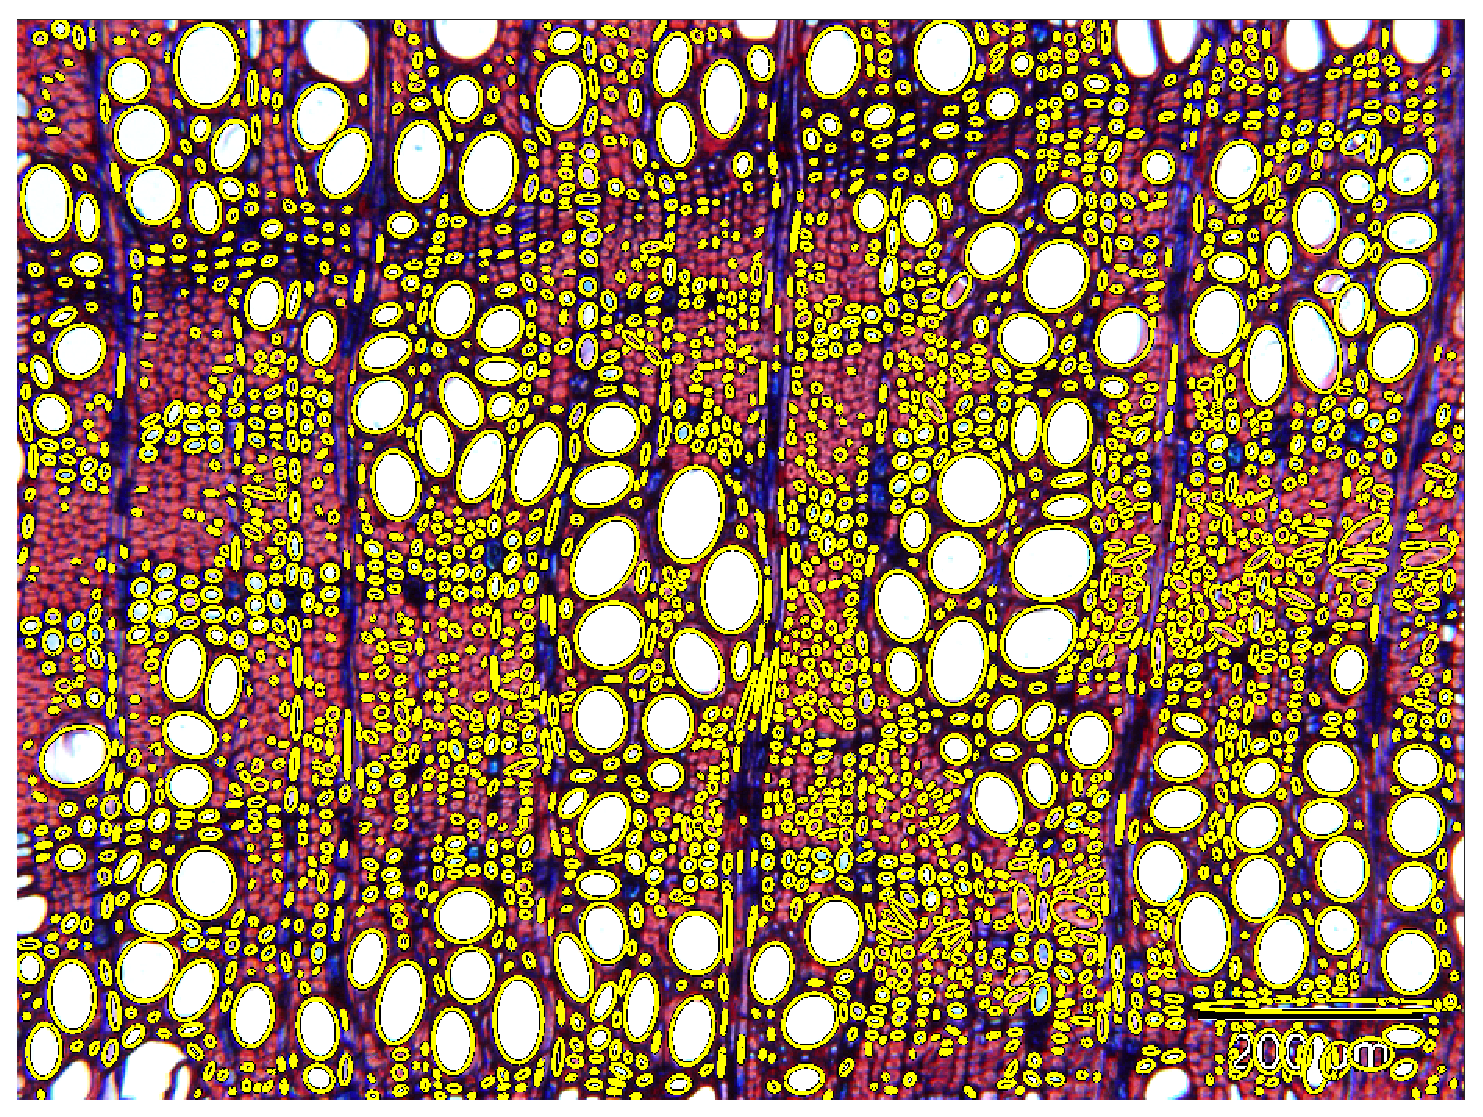
\includegraphics[width=4.0cm]{./Figs/dmsrWood}}
 % \vspace{0.2cm}
 % \centerline{(b) DMSR}\medskip
\end{minipage}
%\vspace{-0.25cm}
\caption{Salient region detectors on microscopy wood images. Left: MSER (every second region is shown), right: DMSR}
\label{fig:wood}
%
\end{figure}
%\vspace{-0.5cm}
%------------------------------------------------------------------------
\begin{figure}[htb]
\centering
\begin{minipage}[b]{.99\linewidth}
  \centering
  \centerline{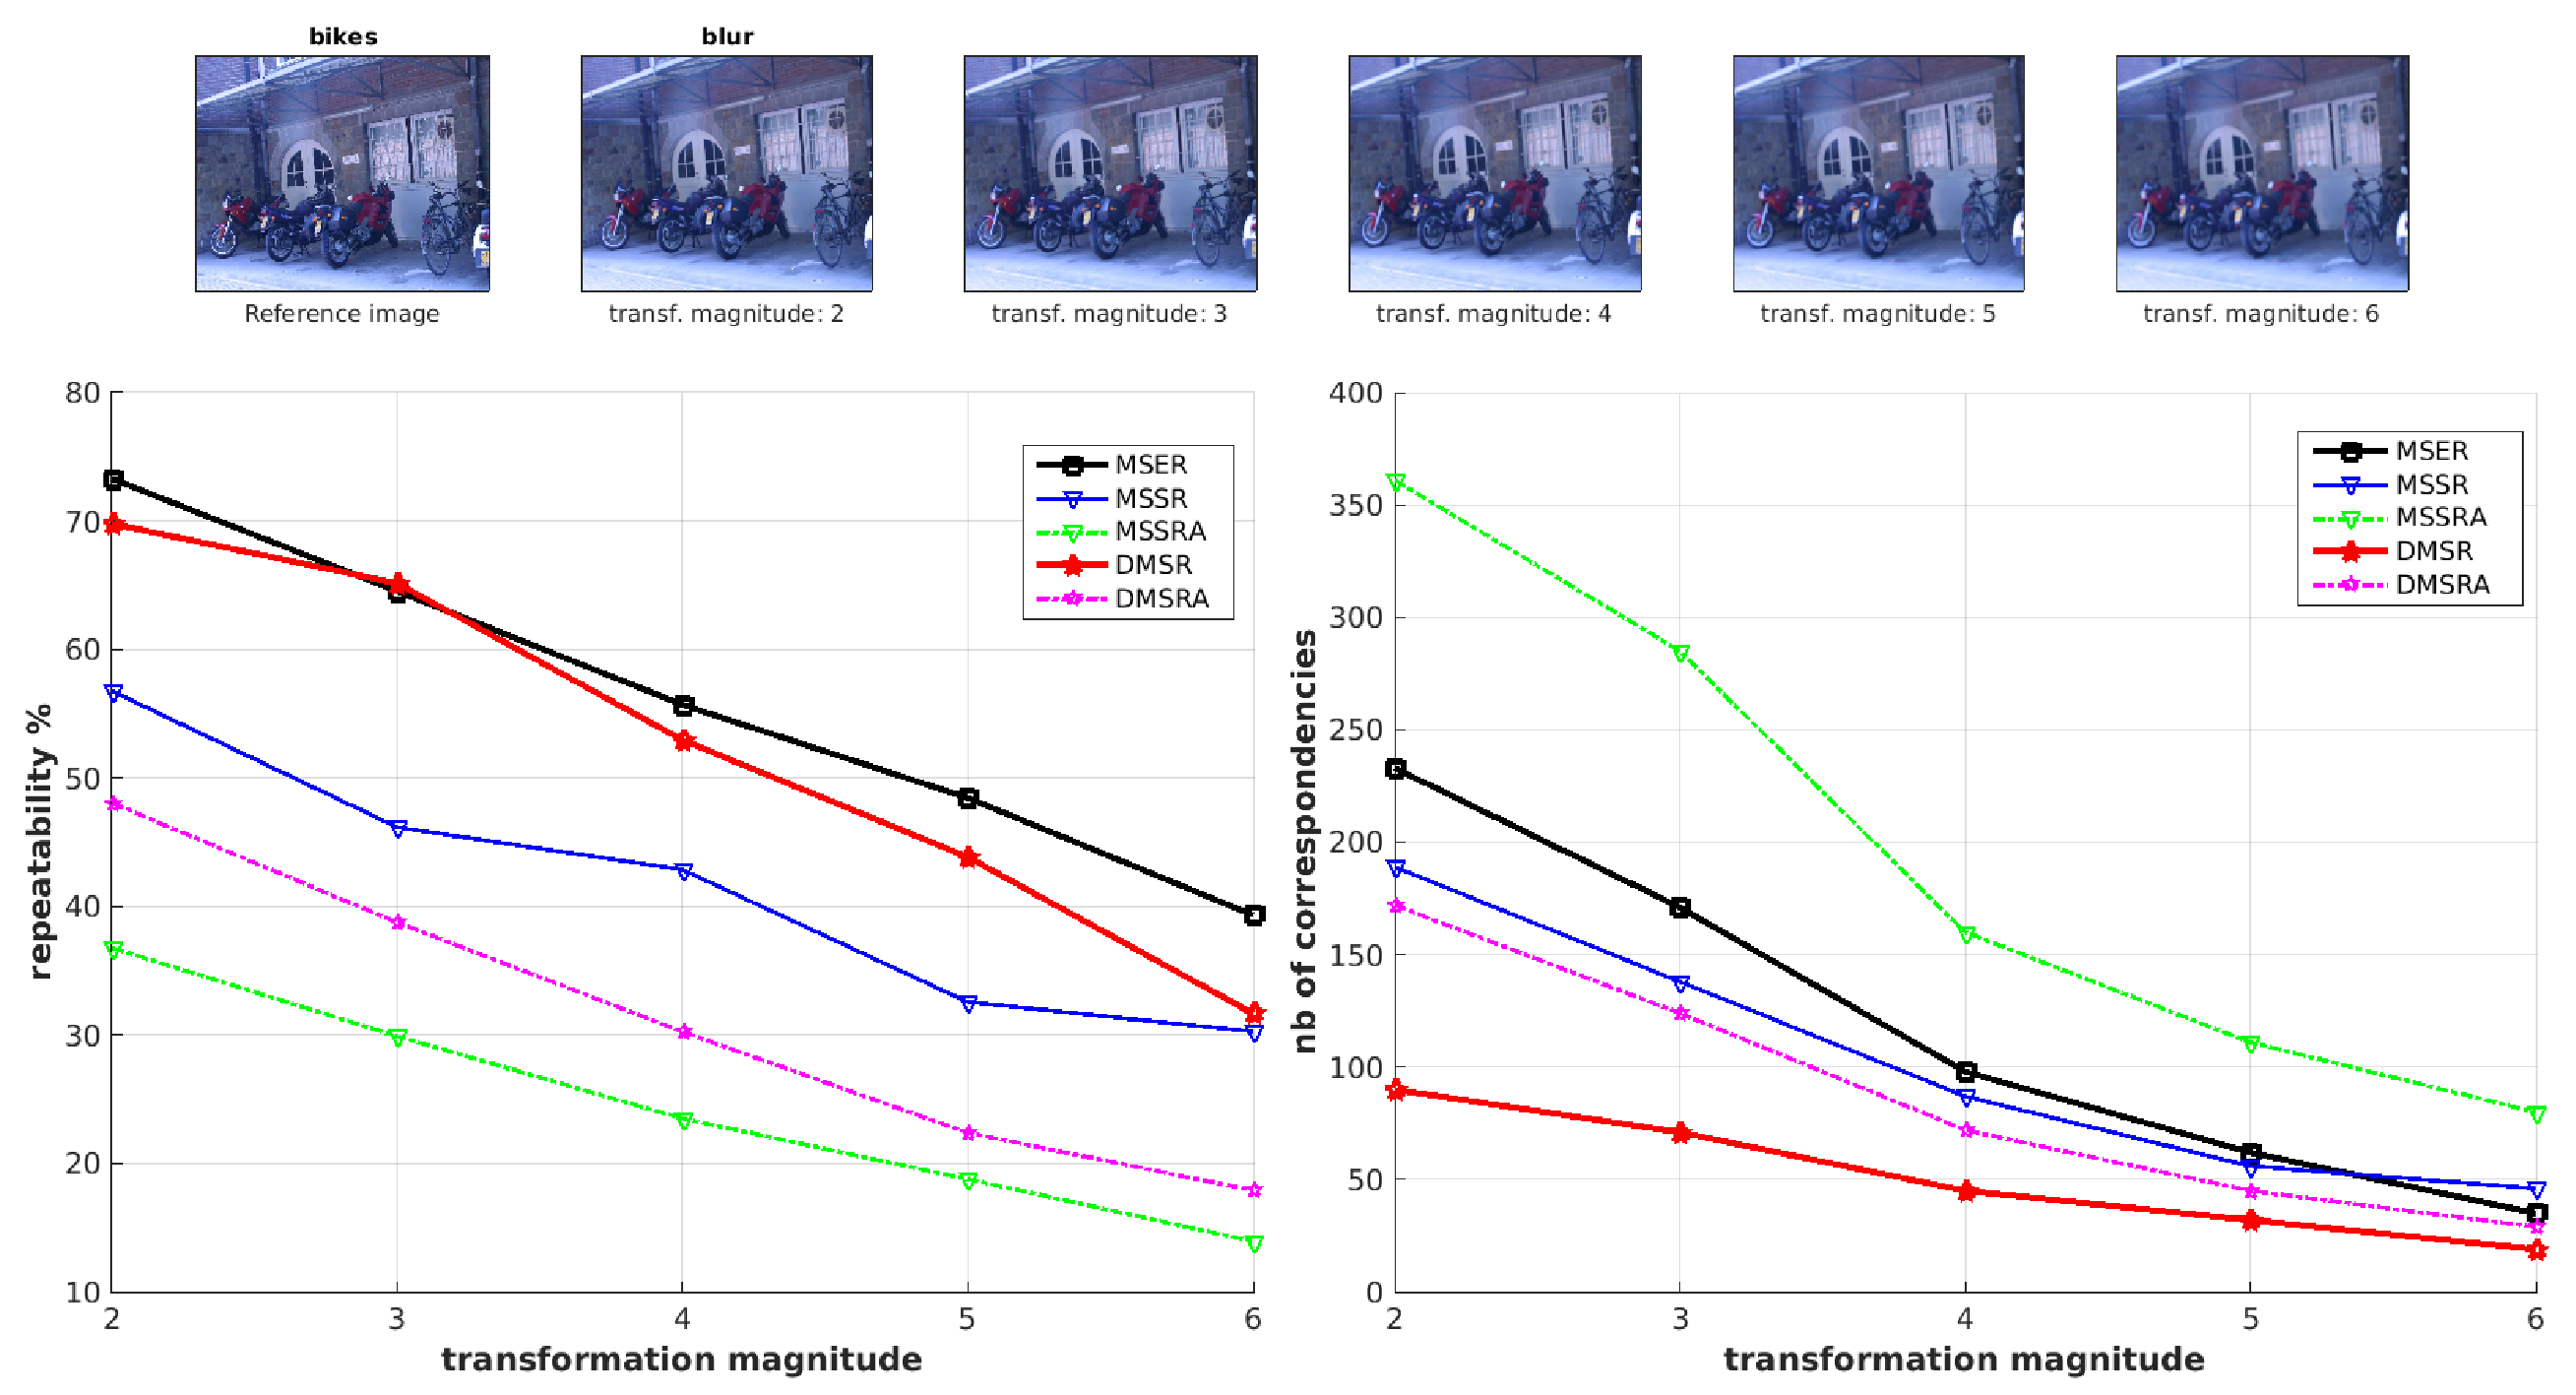
\includegraphics[width=8.5cm]{./Figs/repeatability_all_affine_bikes_blur}}
 % \vspace{0.2cm}
 % \centerline{(a) MSER}\medskip
\end{minipage}
\hfill
%\vspace{-0.25cm}
\caption{Region detection on 'Bikes', Oxford dataset.}
\label{fig:det_bikes}
%
\end{figure}
%------------------------------------------------------------------------
%\vspace{-0.5cm}
\begin{figure}[htb]
\centering
\begin{minipage}[b]{.99\linewidth}
  \centering
 \centerline{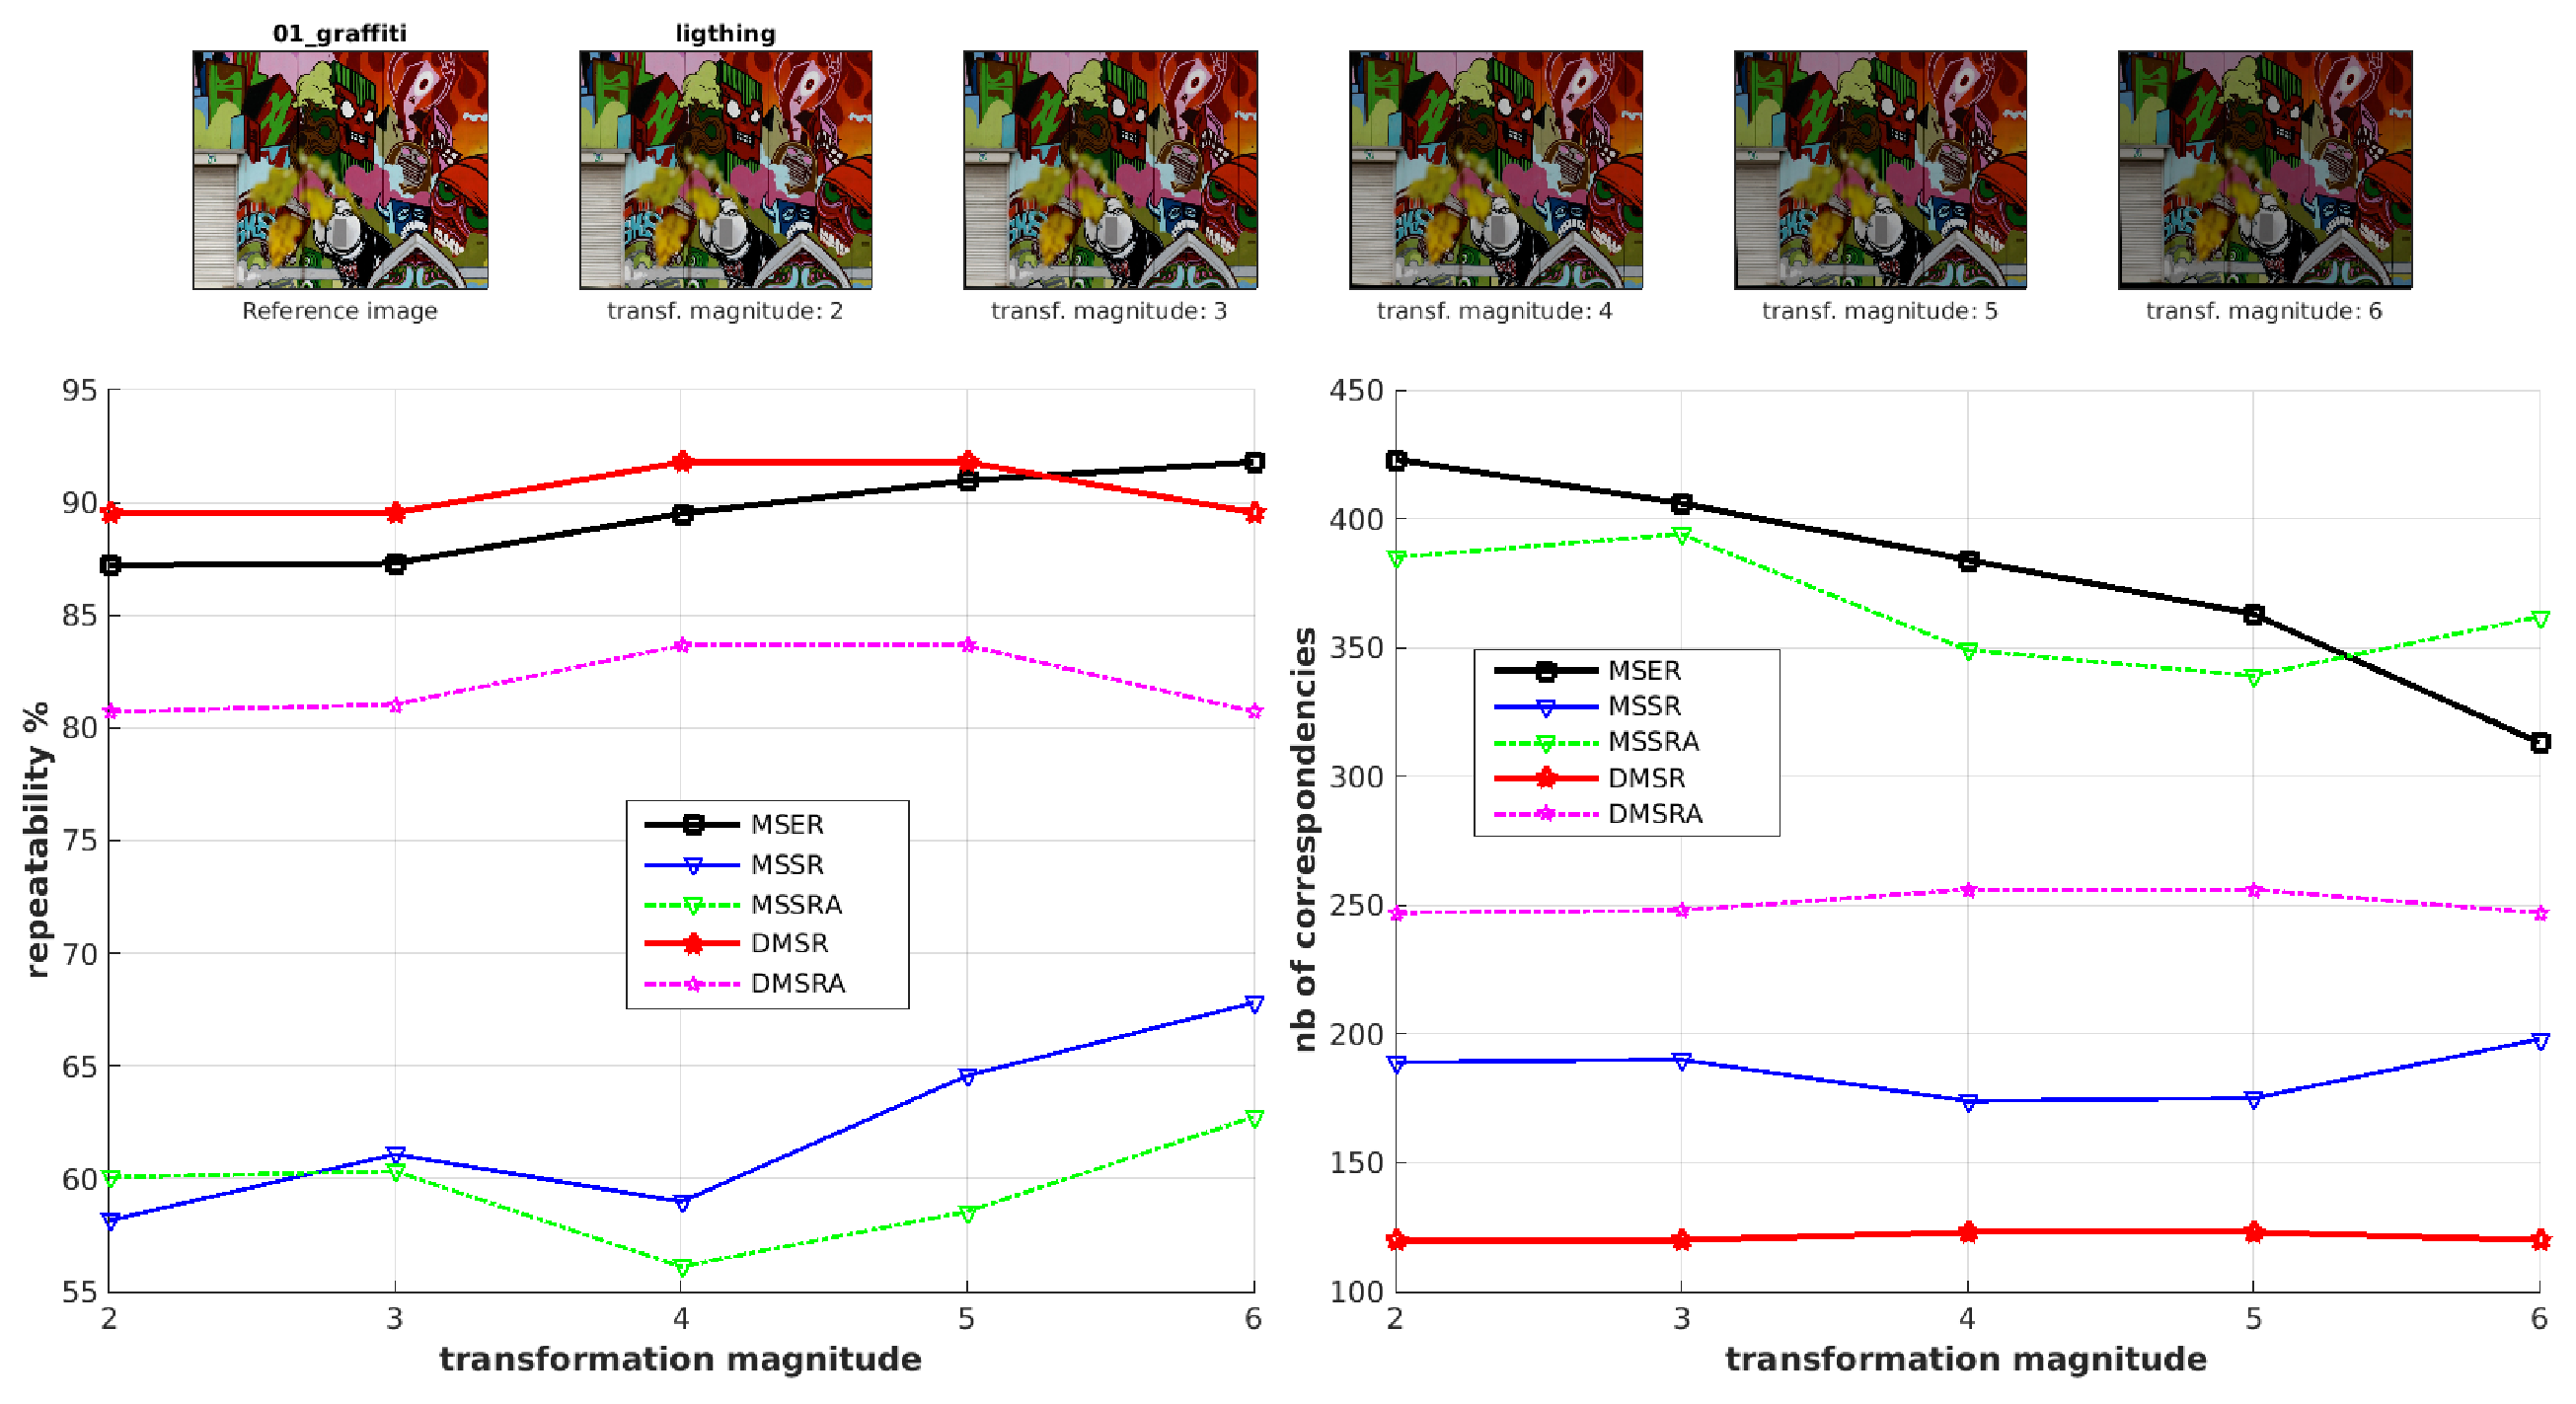
\includegraphics[width=8.5cm]{./Figs/repeatability_all_combined_01_graffiti_ligthing_good}}
 % \vspace{0.2cm}
 % \centerline{(a) MSER}\medskip
\end{minipage}
\hfill
%\vspace{-0.25cm}
\caption{Region detectors on '01\_graffiti', OxFrei dataset.}
\label{fig:det_frei}
%
\end{figure}
%------------------------------------------------------------------------

\begin{figure}[htb]

\begin{minipage}[b]{.9\linewidth}
  \centering
  \centerline{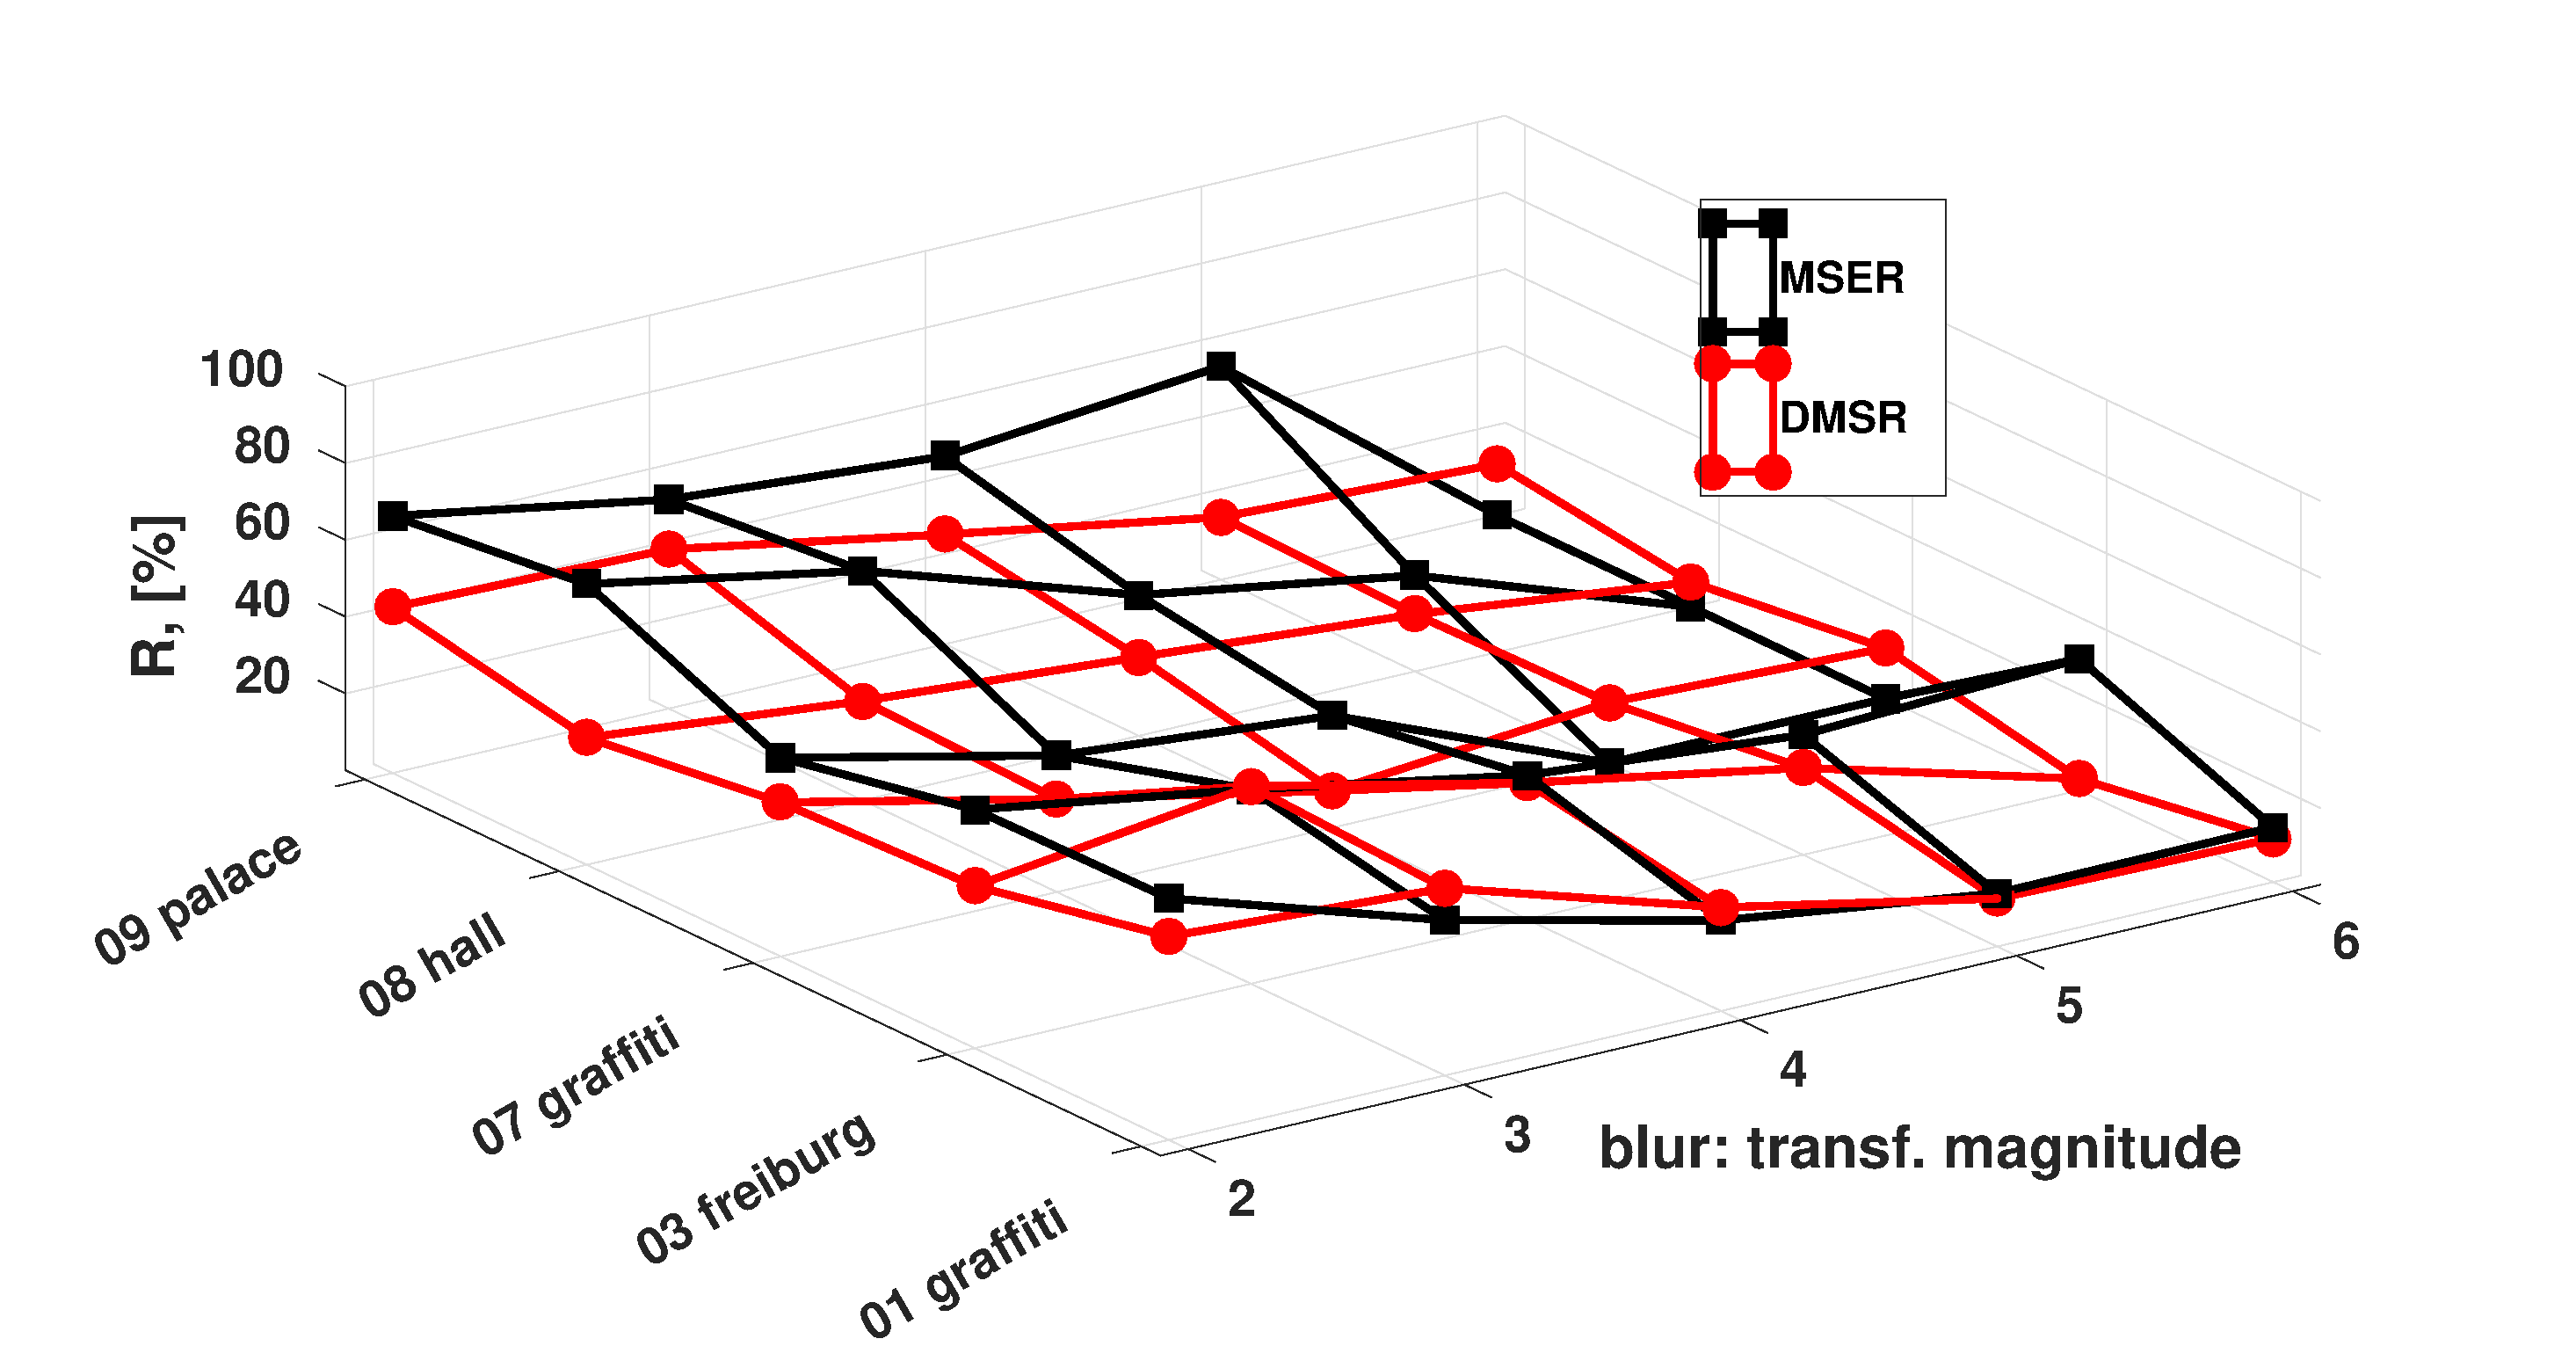
\includegraphics[width=8.5cm]{./Figs/blur_some_combined}}
 % \vspace{0.2cm}
 % \centerline{(a) MSER}\medskip
\end{minipage}
\hfill
%\vspace{-0.25cm}
\caption{Robustness of region detectors to blur on five sequences of the OxFrei dataset.}
\label{fig:blur}
%
\end{figure}
%------------------------------------------------------------------------
%------------------------------------------------------------------------
\subsection{Oxford dataset}
\label{ssec:oxford}
Each image sequence of the Oxford dataset consists of one base and five increasingly distorted images \cite{Mikolajczyk:2005}. They are obtained independently of each other and the homographies between each pair $(\I_B,\I_T)$ are the provided  ground truth. Each sequence can be used to test only one transformation $T$.
For the viewpoint ('Graffiti'), the best $R$ is achieved by DMSR with up to $72\%$, which is $10\%$ more than the second performing MSER for a $40^{\circ}$ change. DMSR is performing worse on the scale ('Boat'), but as good as or better than MSER on the blur ('Bikes', Fig.~\ref{fig:det_bikes}) and lighting ('Leuven') sequences.

\subsection{OxFrei dataset}
\label{ssec:combined}
The creators of the Freiburg dataset separated $T$ from the image content by applying a few transformations (alas not fully documented) to different base images \cite{FischerDB14}. To address the shortage of evaluation datasets, we release OxFrei - a combination of the strong features of the Oxford and Freiburg datasets \cite{elena_ranguelova_2016_45156}. We transform the Freiburg base images with all homographies of the Oxford dataset. In this way, we create $54$ images in $9$ structured scenes each under realistic blur, lighting, scaling and viewpoint transformations.

The dataset allows a transformation independent robustness study by comparing performance on all data subject to the same realistic $T$. Figures~\ref{fig:det_frei} and \ref{fig:blur} show $R$ for lighting for one and blur for a few sequences. The standard plots (like on Fig.~\ref{fig:det_frei}) are cross-sections along the data dimension of the 3D plots (like on Fig.~\ref{fig:blur}) for one sequence. The 2D plots for all OxFrei experiments are online \cite{elena_ranguelova_2016_45156}. We conclude that MSER is better for zoom and viewpoint (the latter contradicting with the result on the single Oxford 'Graffiti' sequence), while DMSR is robust to lighting and blur (Fig. \ref{fig:blur}).

\subsection{TNT hi-res benchmark}
\label{ssec:tnt}

The $R$ score of all detectors from the Oxford study drops down on hi-res images \cite{CorRos2013}. On the 'underground' sequence from the TNT set, MSER loses up to $25\%$ between $1.5$~Mpx ($R_1$) and $8$Mpx ($R_4$) resolutions. On the contrary, DMSR increases the $R$ score as resolution increases on 'underground' and 'posters' sequences with up to $75\%$, which is a $15\%$ increase from $R_1$ to $R_4$ for a $40^{\circ}$ viewpoint change (Figure \ref{fig:tnt}). 

\begin{figure}[htb]

\begin{minipage}[b]{.9\linewidth}
  \centering
  \centerline{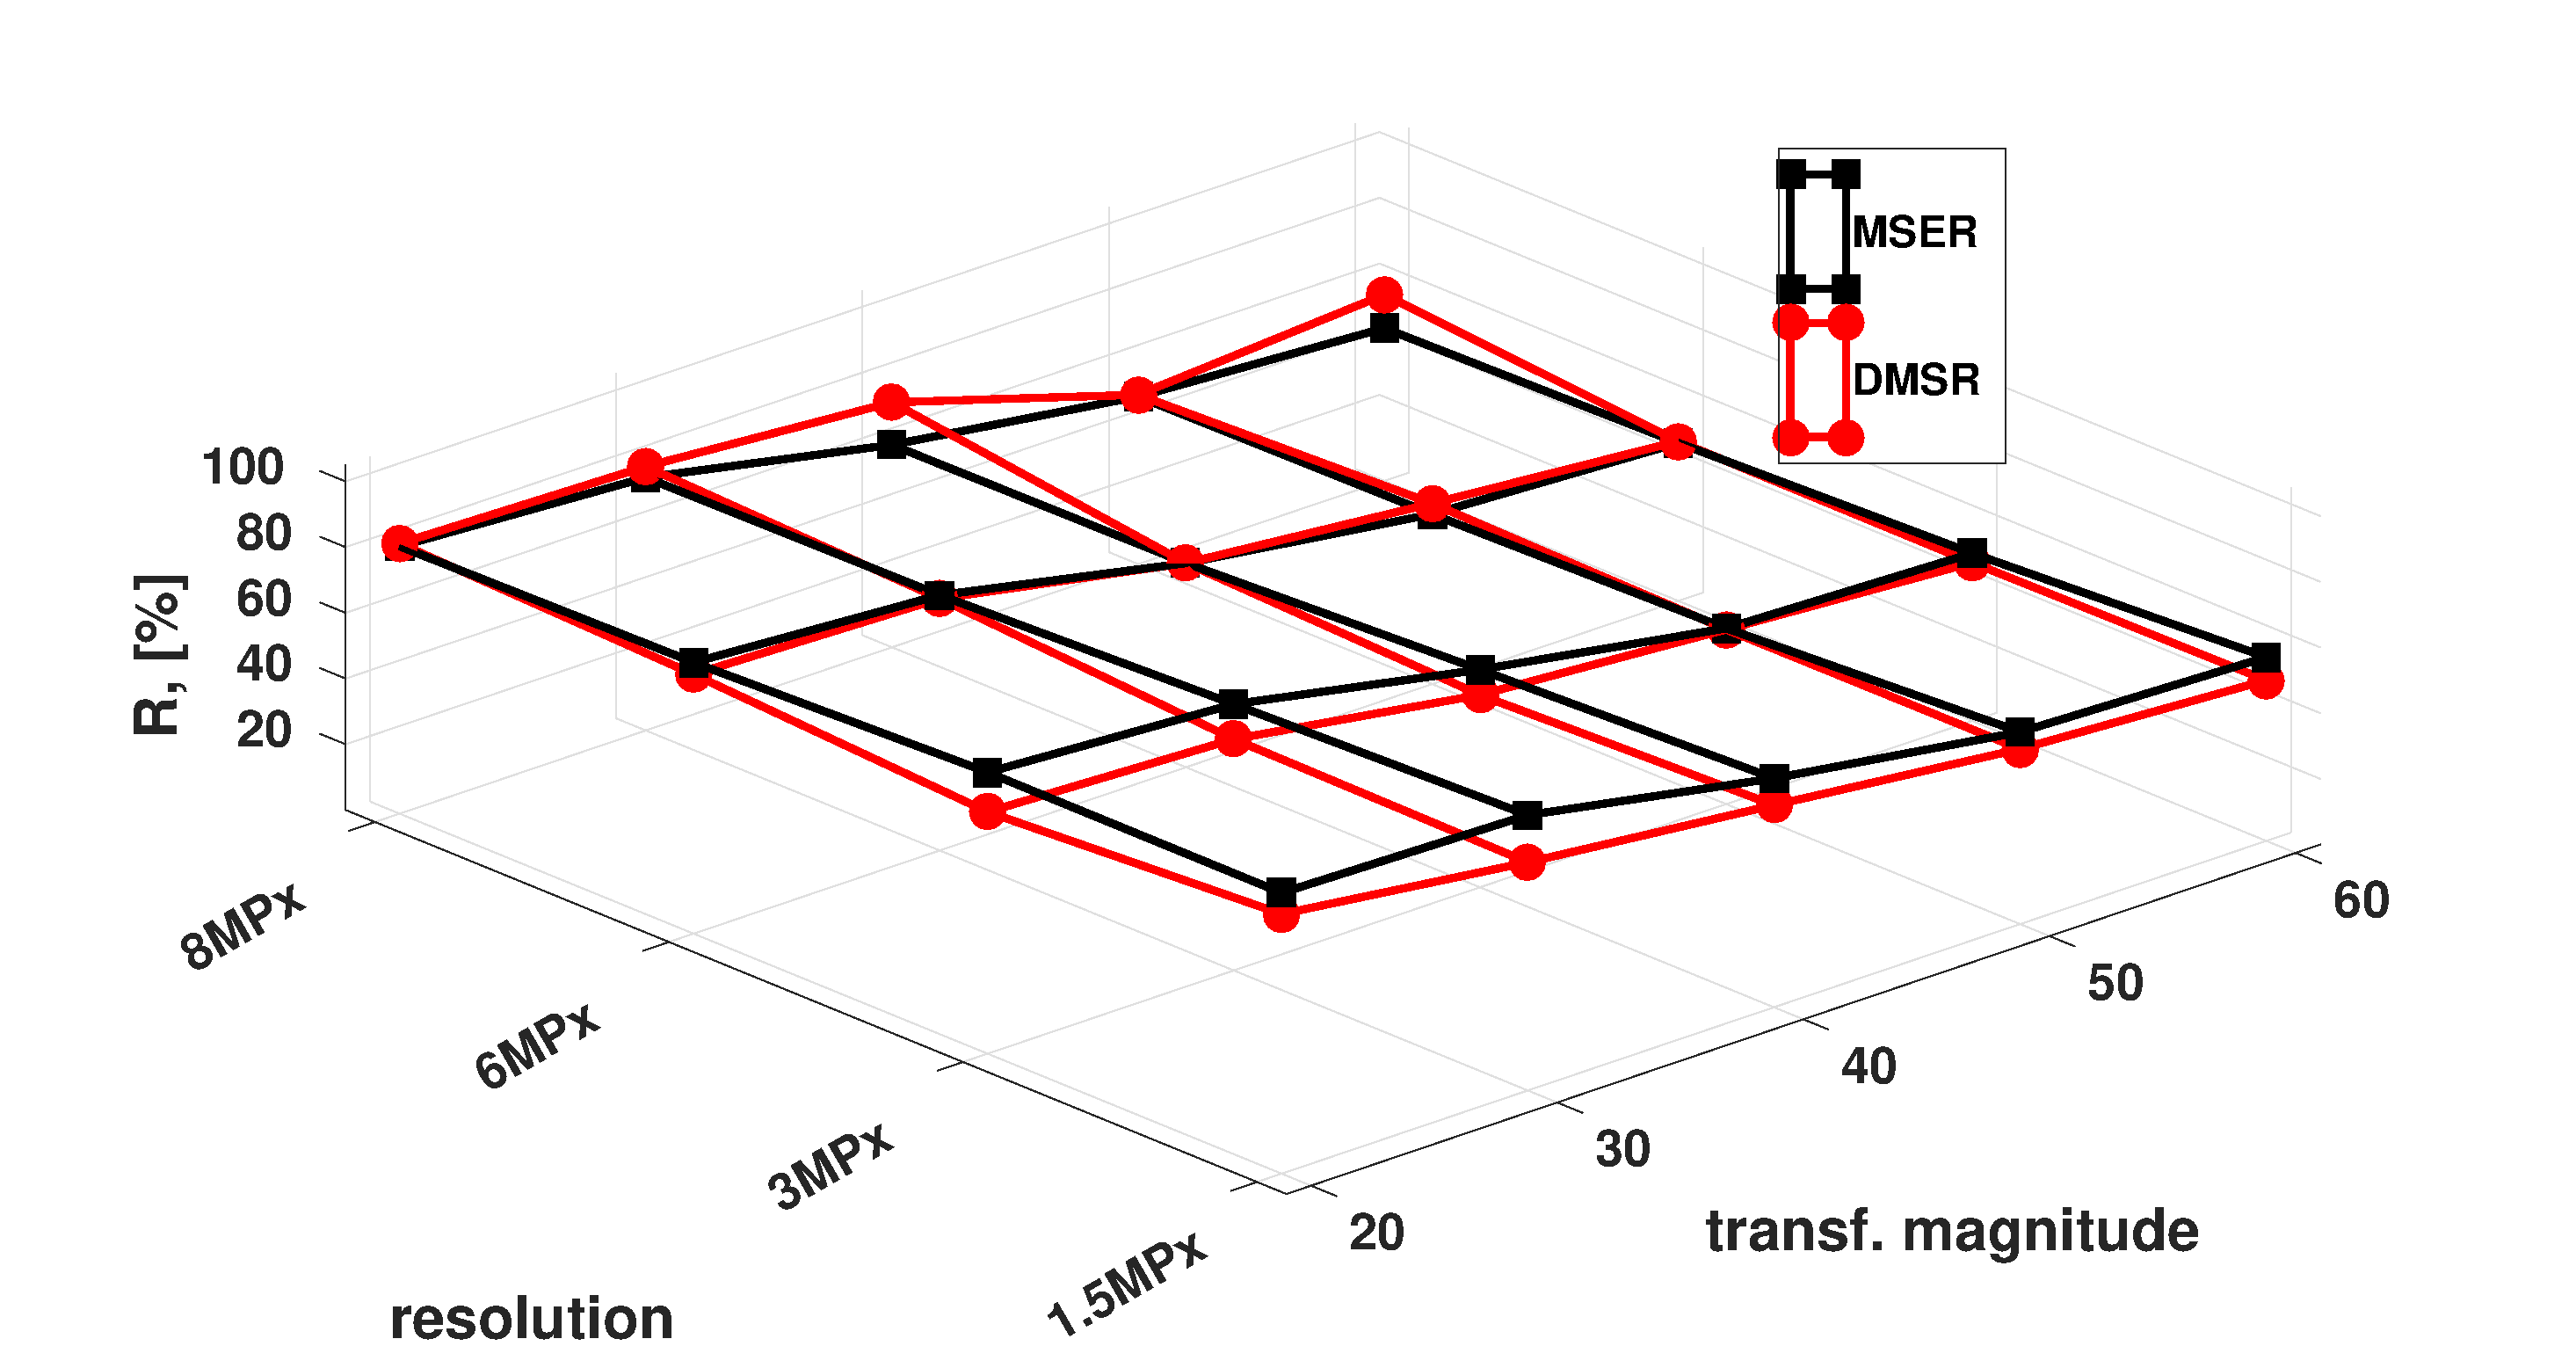
\includegraphics[width=8.5cm]{./Figs/posters_rep}}
 % \vspace{0.2cm}
 % \centerline{(a) MSER}\medskip
\end{minipage}
\hfill
\caption{Robustness of region detectors to image resolution and viewpoint. 'Posters', TNT dataset.}
\label{fig:tnt}
\vspace{-0.25cm}
\end{figure}
%------------------------------------------------------------------------
\begin{figure}[htb]

\begin{minipage}[b]{0.9\linewidth}
  \centering
  \centerline{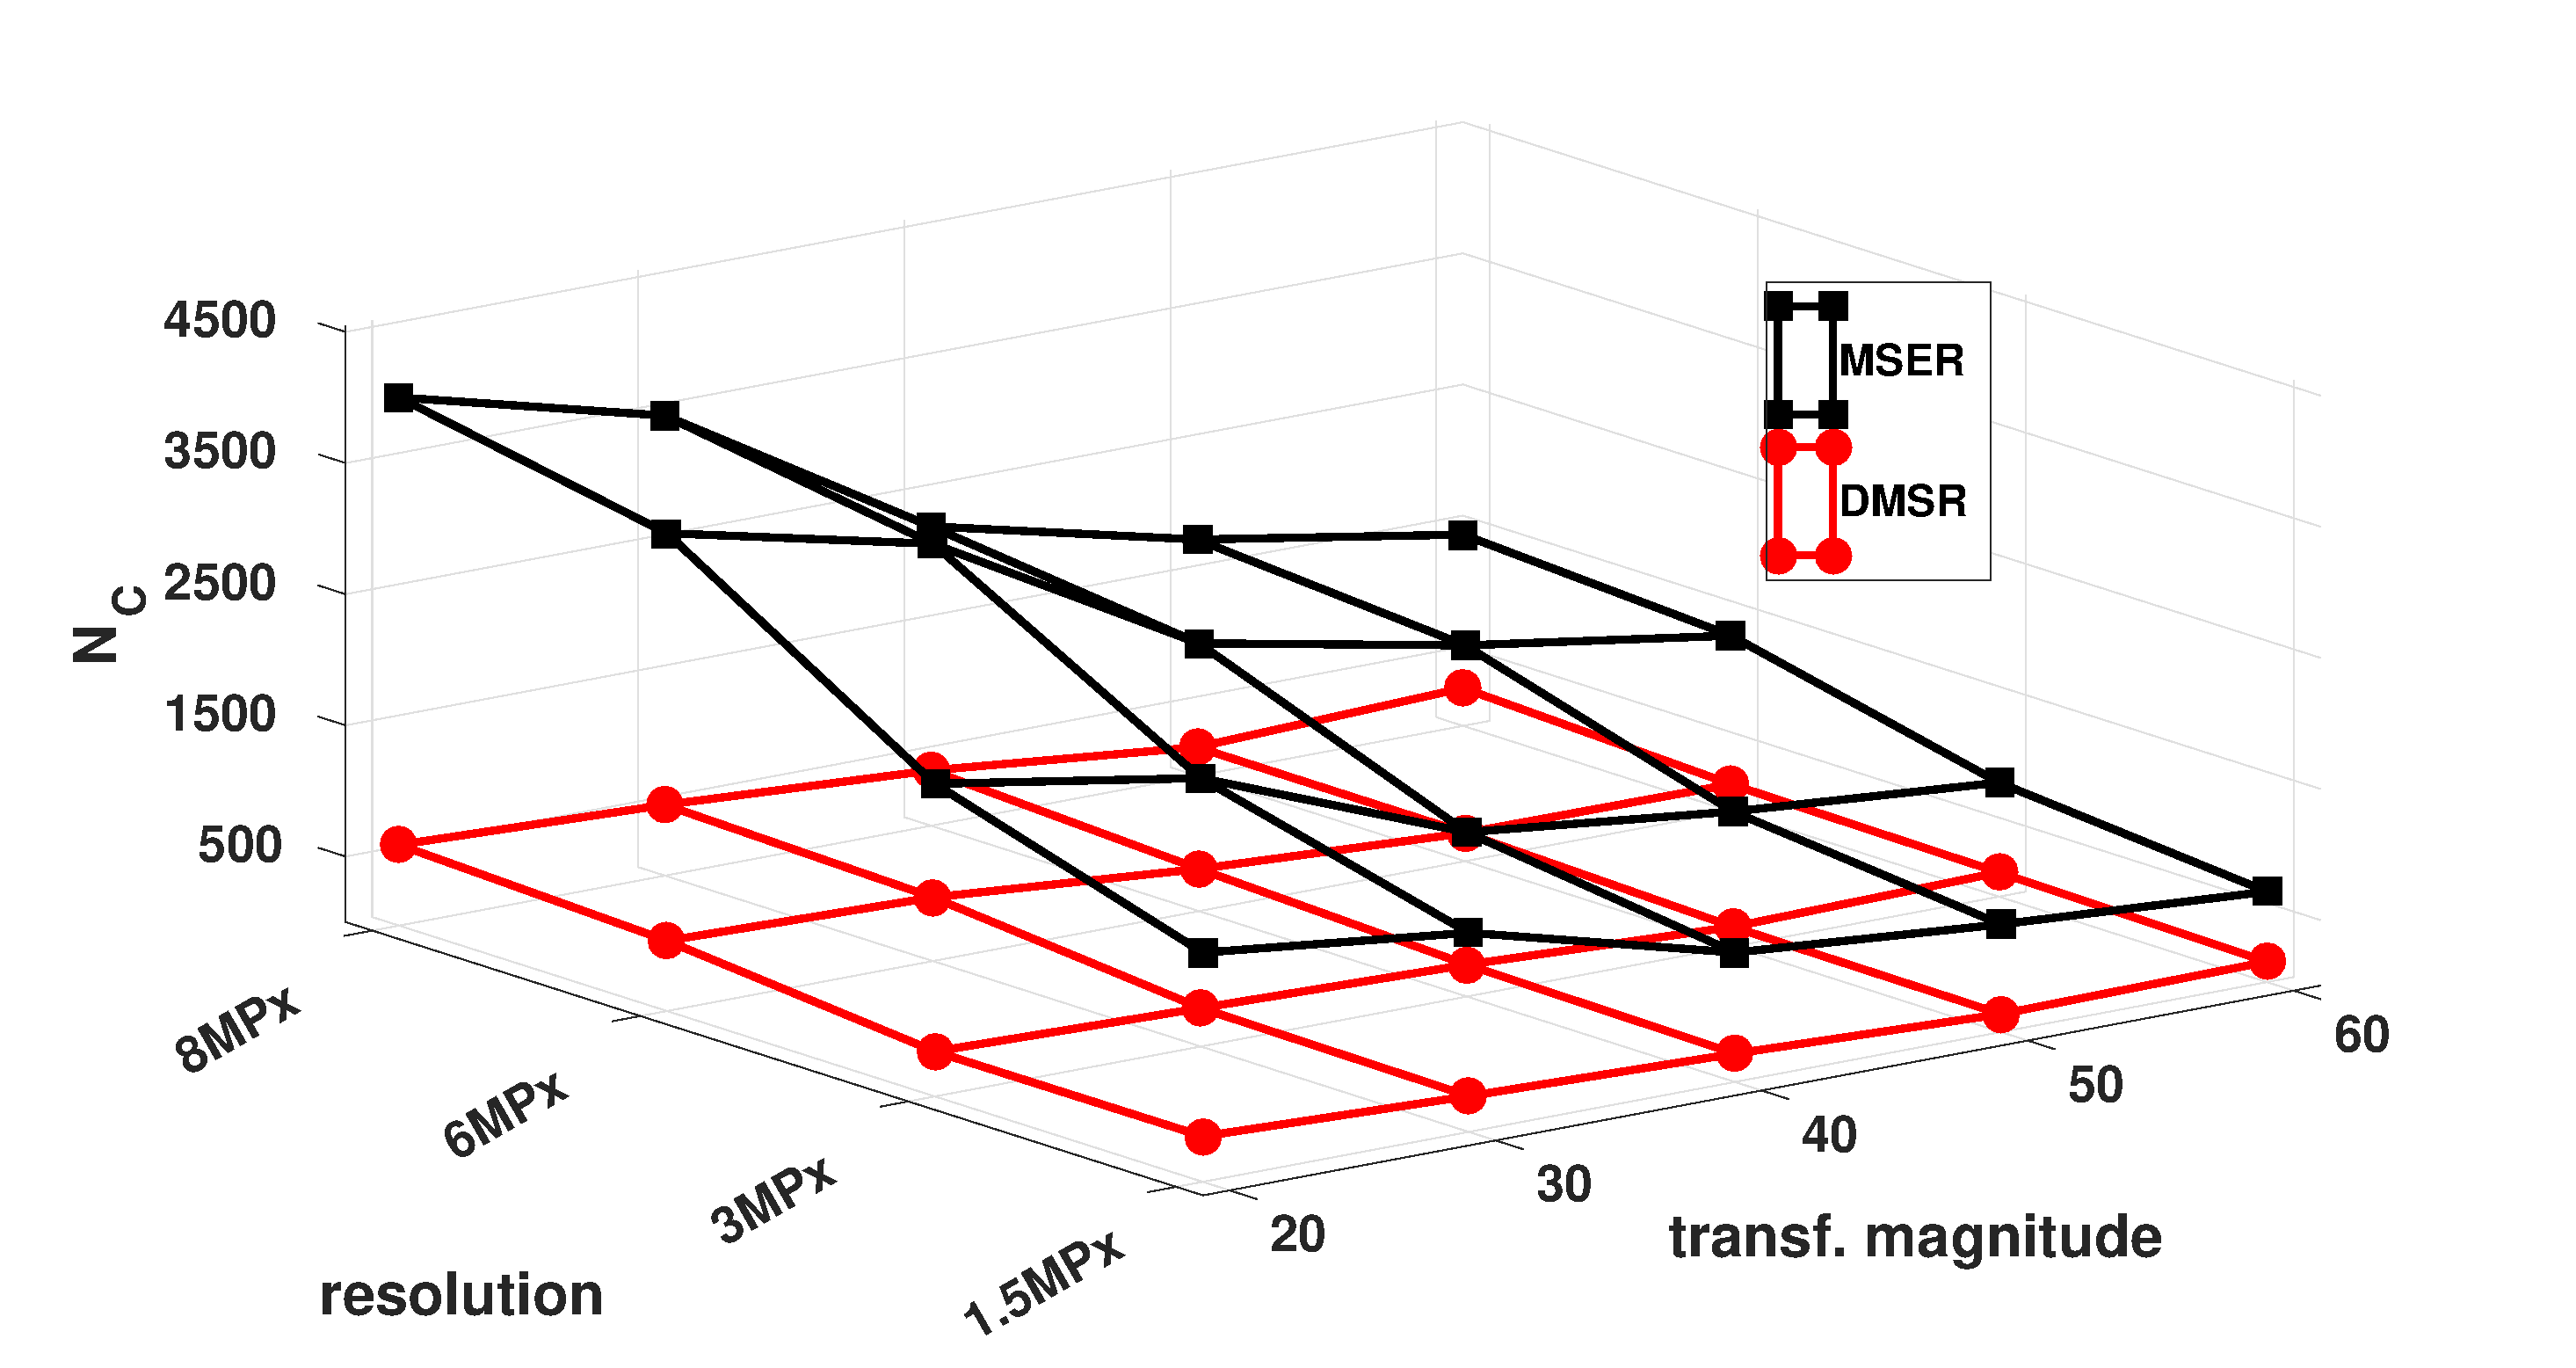
\includegraphics[width=8.5cm]{./Figs/posters_numreg}}
 % \vspace{0.2cm}
 % \centerline{(b) DMSR}\medskip
\end{minipage}
%\vspace{-0.25cm}
\caption{Number of region correspondences versus image resolution and viewpoint. 'Posters', TNT dataset.}
\label{fig:tnt_numreg}
%
\end{figure}
%------------------------------------------------------------------------


\subsection{Animal and plant biometrics}
\label{ssec:bio}
The DMSR detector has been compared to MSER on several small animal individual photo-ID datasets (humpback whales, leatherback turtles, newts) and on a wood species identification dataset \cite{RangHumpb06, PauwelsZB08, wood}. In all cases DMSR produces fewer and perceptually more acurate salient regions as illustrated by Figures~\ref{fig:tails}, \ref{fig:turtle} and \ref{fig:wood}. For the wood microscopy images, it is not possible to obtain accurate statistics on the cell properties with MSER, while the detected DMSR regions enable such wood anatomy research.

On all datasets, the $N_C$ plane of DMSR has the lowest values and the least slope of all detectors (Figs.~\ref{fig:det_bikes}, \ref{fig:det_frei}, right and Fig.~\ref{fig:tnt_numreg}) \cite{elena_ranguelova_2016_45156}. 
The number of detected DMSR regions is up to an order of magnitude lower compared to MSER - crucial for the efficiency of the following matching step on large-scale image data.
Using all $4$ types of regions does not improve performance over using only $ISS$ (holes and islands) with the exception of detecting markings on humpback whale tails. 

\section{CONCLUSIONS}
Combining data-driven binarization with morphological operations yeilds a region detector with comparable to superior performance to MSER on various datasets. DMSR produces a much smaller number of regions- a very desired property in large scale processing. It copes better with blur, lighting and increased resolution and detects perceptually salient regions, which makes it a good choice for scientific imagery analytics. 
For detection evaluation, high-resolution transformation-independent datasets should become the standard.
\label{sec:concl}




% To start a new column (but not a new page) and help balance the last-page
% column length use \vfill\pagebreak.
% -------------------------------------------------------------------------
%\vfill
%\pagebreak


%\section{REFERENCES}
%\label{sec:ref}


% References should be produced using the bibtex program from suitable
% BiBTeX files (here: strings, refs, manuals). The IEEEbib.bst bibliography
% style file from IEEE produces unsorted bibliography list.
% -------------------------------------------------------------------------
\bibliographystyle{IEEEbib}
\bibliography{icip2016}

\end{document}
